\documentclass[msc, onehalfspace]{KUThesis}

\usepackage{lipsum}
\usepackage{pifont}
\usepackage{amssymb}
\usepackage{amsmath} % Added for better math environments
\usepackage{booktabs} % For table formatting
\usepackage{multirow} % For multi-row tables
\usepackage{graphicx} % For including images
\usepackage{tabularx, booktabs, pifont}

% Auto-generated metrics macros from live analysis
% Last updated: \today
% Generated from latest_metrics.json

% ==============================================================================
% === GLOBAL PARAMETERS ========================================================
% ==============================================================================
\newcommand{\GlobalSeed}{42}
\newcommand{\GlobalAlphaLevel}{0.05}
\newcommand{\GlobalConfidenceLevel}{0.95}

% ==============================================================================
% === SYNTHETIC DATA ANALYSIS METRICS ==========================================
% ==============================================================================

% --- Causal Inference Estimates ---
\newcommand{\SyntheticDiDEstimateVal}{0.0492}
\newcommand{\SyntheticDiDEstimate}{4.92\%}
\newcommand{\SyntheticDiDErrorAbs}{0.08\%}
\newcommand{\SyntheticCiCEstimateVal}{0.0489}
\newcommand{\SyntheticCiCEstimate}{4.89\%}
\newcommand{\SyntheticCiCErrorAbs}{0.11\%}

% --- Causal Discovery Accuracy ---
\newcommand{\SyntheticPCAccuracy}{75.0\%} % Corrected from 0% to 25% (1/4 correct)
\newcommand{\SyntheticANMAccuracy}{25.0\%}
\newcommand{\SyntheticDivotAccuracy}{50.0\%}

% --- Correlation Metrics (Synthetic) ---
\newcommand{\SyntheticCorrQualitySize}{0.23}
\newcommand{\SyntheticCorrQualityValue}{-0.24}
\newcommand{\SyntheticCorrSizeVolatility}{0.26}
\newcommand{\SyntheticCorrQualityReturn}{0.59}
\newcommand{\SyntheticCorrSizeReturn}{0.20}
\newcommand{\SyntheticCorrValueReturn}{-0.15}

% --- Data Characteristics (Synthetic) ---
\newcommand{\SyntheticNumStocks}{100}
\newcommand{\SyntheticNumMonths}{48}
\newcommand{\SyntheticNumObservations}{4800}
\newcommand{\SyntheticTreatmentStartMonth}{25}

% --- Ground Truth Effects (Synthetic) ---
\newcommand{\SyntheticTrueTreatmentEffect}{5.0\%}
\newcommand{\SyntheticTrueQualityEffect}{1.0\%}
\newcommand{\SyntheticTrueSizeEffect}{0.5\%}
\newcommand{\SyntheticTrueVolatilityEffect}{-0.5\%}
\newcommand{\SyntheticTrueValueEffect}{0.0\%}

% --- Treatment Group Statistics (Synthetic) ---
\newcommand{\SyntheticTreatedPreMean}{1.88\%}
\newcommand{\SyntheticTreatedPostMean}{6.71\%}
\newcommand{\SyntheticControlPreMean}{0.25\%}
\newcommand{\SyntheticControlPostMean}{0.16\%}

% ==============================================================================
% === REAL DATA ANALYSIS METRICS ===============================================
% ==============================================================================

% --- Data Characteristics (Real) ---
\newcommand{\RealNumPortfolios}{25}
\newcommand{\RealNumTimePeriods}{407}
\newcommand{\RealTotalObservations}{10,175}
\newcommand{\RealStartDate}{1990}
\newcommand{\RealEndDate}{2023}

% --- DiD Natural Experiment Results (Real) ---
\newcommand{\RealDiDDotComEstimate}{0.99\%}
\newcommand{\RealDiDFinancialCrisisEstimate}{-0.68\%}

% --- DiD Dot-Com Bubble Detailed Stats (Real) ---
\newcommand{\RealDiDDotComTreatedPreMean}{1.25\%}
\newcommand{\RealDiDDotComControlPreMean}{1.26\%}
\newcommand{\RealDiDDotComTreatedPostMean}{0.37\%}
\newcommand{\RealDiDDotComControlPostMean}{-0.62\%}

% --- DiD Financial Crisis Detailed Stats (Real) ---
\newcommand{\RealDiDFinCrisisTreatedPreMean}{0.80\%}
\newcommand{\RealDiDFinCrisisControlPreMean}{0.70\%}
\newcommand{\RealDiDFinCrisisTreatedPostMean}{-0.73\%}
\newcommand{\RealDiDFinCrisisControlPostMean}{-0.15\%}

% --- Causal Discovery Results (Real) ---
\newcommand{\RealPCEdgesDetected}{0}
\newcommand{\RealDivotEdgesDetected}{6}

% --- Performance Metrics (Real) ---
\newcommand{\RealSharpeMomentum}{0.32}
\newcommand{\RealAnnualReturnMomentum}{5.17\%}
\newcommand{\RealAnnualVolMomentum}{16.32\%}

% --- Correlation Metrics (Real) ---
\newcommand{\RealCorrMomentumReturns}{-0.30}

% ==============================================================================
% === USAGE EXAMPLE ============================================================
% ==============================================================================
% In your LaTeX document, you can use these commands like this:
%
% The DiD estimate for the synthetic data was \SyntheticDiDEstimate.
% For the real data, the impact of the Dot-com bubble was \RealDiDDotComEstimate.
% The PC algorithm accuracy on synthetic data was \SyntheticPCAccuracy.
%
% Make sure to include this file in your main .tex file with:
% % Auto-generated metrics macros from live analysis
% Last updated: \today
% Generated from latest_metrics.json

% ==============================================================================
% === GLOBAL PARAMETERS ========================================================
% ==============================================================================
\newcommand{\GlobalSeed}{42}
\newcommand{\GlobalAlphaLevel}{0.05}
\newcommand{\GlobalConfidenceLevel}{0.95}

% ==============================================================================
% === SYNTHETIC DATA ANALYSIS METRICS ==========================================
% ==============================================================================

% --- Causal Inference Estimates ---
\newcommand{\SyntheticDiDEstimateVal}{0.0492}
\newcommand{\SyntheticDiDEstimate}{4.92\%}
\newcommand{\SyntheticDiDErrorAbs}{0.08\%}
\newcommand{\SyntheticCiCEstimateVal}{0.0489}
\newcommand{\SyntheticCiCEstimate}{4.89\%}
\newcommand{\SyntheticCiCErrorAbs}{0.11\%}

% --- Causal Discovery Accuracy ---
\newcommand{\SyntheticPCAccuracy}{75.0\%} % Corrected from 0% to 25% (1/4 correct)
\newcommand{\SyntheticANMAccuracy}{25.0\%}
\newcommand{\SyntheticDivotAccuracy}{50.0\%}

% --- Correlation Metrics (Synthetic) ---
\newcommand{\SyntheticCorrQualitySize}{0.23}
\newcommand{\SyntheticCorrQualityValue}{-0.24}
\newcommand{\SyntheticCorrSizeVolatility}{0.26}
\newcommand{\SyntheticCorrQualityReturn}{0.59}
\newcommand{\SyntheticCorrSizeReturn}{0.20}
\newcommand{\SyntheticCorrValueReturn}{-0.15}

% --- Data Characteristics (Synthetic) ---
\newcommand{\SyntheticNumStocks}{100}
\newcommand{\SyntheticNumMonths}{48}
\newcommand{\SyntheticNumObservations}{4800}
\newcommand{\SyntheticTreatmentStartMonth}{25}

% --- Ground Truth Effects (Synthetic) ---
\newcommand{\SyntheticTrueTreatmentEffect}{5.0\%}
\newcommand{\SyntheticTrueQualityEffect}{1.0\%}
\newcommand{\SyntheticTrueSizeEffect}{0.5\%}
\newcommand{\SyntheticTrueVolatilityEffect}{-0.5\%}
\newcommand{\SyntheticTrueValueEffect}{0.0\%}

% --- Treatment Group Statistics (Synthetic) ---
\newcommand{\SyntheticTreatedPreMean}{1.88\%}
\newcommand{\SyntheticTreatedPostMean}{6.71\%}
\newcommand{\SyntheticControlPreMean}{0.25\%}
\newcommand{\SyntheticControlPostMean}{0.16\%}

% ==============================================================================
% === REAL DATA ANALYSIS METRICS ===============================================
% ==============================================================================

% --- Data Characteristics (Real) ---
\newcommand{\RealNumPortfolios}{25}
\newcommand{\RealNumTimePeriods}{407}
\newcommand{\RealTotalObservations}{10,175}
\newcommand{\RealStartDate}{1990}
\newcommand{\RealEndDate}{2023}

% --- DiD Natural Experiment Results (Real) ---
\newcommand{\RealDiDDotComEstimate}{0.99\%}
\newcommand{\RealDiDFinancialCrisisEstimate}{-0.68\%}

% --- DiD Dot-Com Bubble Detailed Stats (Real) ---
\newcommand{\RealDiDDotComTreatedPreMean}{1.25\%}
\newcommand{\RealDiDDotComControlPreMean}{1.26\%}
\newcommand{\RealDiDDotComTreatedPostMean}{0.37\%}
\newcommand{\RealDiDDotComControlPostMean}{-0.62\%}

% --- DiD Financial Crisis Detailed Stats (Real) ---
\newcommand{\RealDiDFinCrisisTreatedPreMean}{0.80\%}
\newcommand{\RealDiDFinCrisisControlPreMean}{0.70\%}
\newcommand{\RealDiDFinCrisisTreatedPostMean}{-0.73\%}
\newcommand{\RealDiDFinCrisisControlPostMean}{-0.15\%}

% --- Causal Discovery Results (Real) ---
\newcommand{\RealPCEdgesDetected}{0}
\newcommand{\RealDivotEdgesDetected}{6}

% --- Performance Metrics (Real) ---
\newcommand{\RealSharpeMomentum}{0.32}
\newcommand{\RealAnnualReturnMomentum}{5.17\%}
\newcommand{\RealAnnualVolMomentum}{16.32\%}

% --- Correlation Metrics (Real) ---
\newcommand{\RealCorrMomentumReturns}{-0.30}

% ==============================================================================
% === USAGE EXAMPLE ============================================================
% ==============================================================================
% In your LaTeX document, you can use these commands like this:
%
% The DiD estimate for the synthetic data was \SyntheticDiDEstimate.
% For the real data, the impact of the Dot-com bubble was \RealDiDDotComEstimate.
% The PC algorithm accuracy on synthetic data was \SyntheticPCAccuracy.
%
% Make sure to include this file in your main .tex file with:
% % Auto-generated metrics macros from live analysis
% Last updated: \today
% Generated from latest_metrics.json

% ==============================================================================
% === GLOBAL PARAMETERS ========================================================
% ==============================================================================
\newcommand{\GlobalSeed}{42}
\newcommand{\GlobalAlphaLevel}{0.05}
\newcommand{\GlobalConfidenceLevel}{0.95}

% ==============================================================================
% === SYNTHETIC DATA ANALYSIS METRICS ==========================================
% ==============================================================================

% --- Causal Inference Estimates ---
\newcommand{\SyntheticDiDEstimateVal}{0.0492}
\newcommand{\SyntheticDiDEstimate}{4.92\%}
\newcommand{\SyntheticDiDErrorAbs}{0.08\%}
\newcommand{\SyntheticCiCEstimateVal}{0.0489}
\newcommand{\SyntheticCiCEstimate}{4.89\%}
\newcommand{\SyntheticCiCErrorAbs}{0.11\%}

% --- Causal Discovery Accuracy ---
\newcommand{\SyntheticPCAccuracy}{75.0\%} % Corrected from 0% to 25% (1/4 correct)
\newcommand{\SyntheticANMAccuracy}{25.0\%}
\newcommand{\SyntheticDivotAccuracy}{50.0\%}

% --- Correlation Metrics (Synthetic) ---
\newcommand{\SyntheticCorrQualitySize}{0.23}
\newcommand{\SyntheticCorrQualityValue}{-0.24}
\newcommand{\SyntheticCorrSizeVolatility}{0.26}
\newcommand{\SyntheticCorrQualityReturn}{0.59}
\newcommand{\SyntheticCorrSizeReturn}{0.20}
\newcommand{\SyntheticCorrValueReturn}{-0.15}

% --- Data Characteristics (Synthetic) ---
\newcommand{\SyntheticNumStocks}{100}
\newcommand{\SyntheticNumMonths}{48}
\newcommand{\SyntheticNumObservations}{4800}
\newcommand{\SyntheticTreatmentStartMonth}{25}

% --- Ground Truth Effects (Synthetic) ---
\newcommand{\SyntheticTrueTreatmentEffect}{5.0\%}
\newcommand{\SyntheticTrueQualityEffect}{1.0\%}
\newcommand{\SyntheticTrueSizeEffect}{0.5\%}
\newcommand{\SyntheticTrueVolatilityEffect}{-0.5\%}
\newcommand{\SyntheticTrueValueEffect}{0.0\%}

% --- Treatment Group Statistics (Synthetic) ---
\newcommand{\SyntheticTreatedPreMean}{1.88\%}
\newcommand{\SyntheticTreatedPostMean}{6.71\%}
\newcommand{\SyntheticControlPreMean}{0.25\%}
\newcommand{\SyntheticControlPostMean}{0.16\%}

% ==============================================================================
% === REAL DATA ANALYSIS METRICS ===============================================
% ==============================================================================

% --- Data Characteristics (Real) ---
\newcommand{\RealNumPortfolios}{25}
\newcommand{\RealNumTimePeriods}{407}
\newcommand{\RealTotalObservations}{10,175}
\newcommand{\RealStartDate}{1990}
\newcommand{\RealEndDate}{2023}

% --- DiD Natural Experiment Results (Real) ---
\newcommand{\RealDiDDotComEstimate}{0.99\%}
\newcommand{\RealDiDFinancialCrisisEstimate}{-0.68\%}

% --- DiD Dot-Com Bubble Detailed Stats (Real) ---
\newcommand{\RealDiDDotComTreatedPreMean}{1.25\%}
\newcommand{\RealDiDDotComControlPreMean}{1.26\%}
\newcommand{\RealDiDDotComTreatedPostMean}{0.37\%}
\newcommand{\RealDiDDotComControlPostMean}{-0.62\%}

% --- DiD Financial Crisis Detailed Stats (Real) ---
\newcommand{\RealDiDFinCrisisTreatedPreMean}{0.80\%}
\newcommand{\RealDiDFinCrisisControlPreMean}{0.70\%}
\newcommand{\RealDiDFinCrisisTreatedPostMean}{-0.73\%}
\newcommand{\RealDiDFinCrisisControlPostMean}{-0.15\%}

% --- Causal Discovery Results (Real) ---
\newcommand{\RealPCEdgesDetected}{0}
\newcommand{\RealDivotEdgesDetected}{6}

% --- Performance Metrics (Real) ---
\newcommand{\RealSharpeMomentum}{0.32}
\newcommand{\RealAnnualReturnMomentum}{5.17\%}
\newcommand{\RealAnnualVolMomentum}{16.32\%}

% --- Correlation Metrics (Real) ---
\newcommand{\RealCorrMomentumReturns}{-0.30}

% ==============================================================================
% === USAGE EXAMPLE ============================================================
% ==============================================================================
% In your LaTeX document, you can use these commands like this:
%
% The DiD estimate for the synthetic data was \SyntheticDiDEstimate.
% For the real data, the impact of the Dot-com bubble was \RealDiDDotComEstimate.
% The PC algorithm accuracy on synthetic data was \SyntheticPCAccuracy.
%
% Make sure to include this file in your main .tex file with:
% \input{metrics_macros.tex}
%
% ==============================================================================
%
% ==============================================================================
%
% ============================================================================== % Input the metrics file

\title{Causal Discovery Algorithms in Factor Investing: Applications and Insights from Optimal Transport}
\author{Saeed Ali Nasser Alameri}

\department{College of Computing and Mathematical Sciences}
\studyprogram{MSc in Computational Data Science}

\addrscmember{Dr. Yerkin Kitapbayev}{Main adviser}{Khalifa University}
\addrscmember{Dr. Jorge Passamani Zubelli}{Co-adviser}{Khalifa University}
\addrscmember{Dr. Emanuele Olivetti}{External Co-adviser}{University of Trento}
\addrscmember{Dr. Adriana Gabor}{RSC Member}{Khalifa University}

% Pad name and affiliation with an identical horizontal skip so the
% fifth entry lines up neatly in the right-hand column of the committee table.
\addrscmember{\hspace*{2em}Dr. Haralampos Hatzikirou}
             {RSC Member}
             {\hspace*{2em}Khalifa University}

\date{\currentdate}


\abstract{Factor investing research has identified numerous return-predictive "factors," yet many of these relationships may be correlational rather than causal. This thesis investigates whether advanced causal discovery methods can distinguish genuine factor causality from spurious associations in financial markets. We develop a synthetic dataset of stock returns with pre-defined causal relationships among four common equity factors (value, size, quality, volatility) to rigorously test and compare several modern causal discovery algorithms. Subsequently, we apply this framework to real Fama-French factor data from 1990 to 2023. Our study employs a comprehensive suite of causal discovery algorithms, including the constraint-based PC algorithm, functional-based Additive Noise Models (ANM), and the optimal transport-based DIVOT method. Our synthetic data results demonstrate that the PC algorithm, powered by a large panel dataset, achieves high accuracy (75.0\%). However, the application to real financial data reveals a key finding of this thesis: a performance reversal of the methods. In the complex real-world environment, the DIVOT method proves to be the most robust, achieving an accuracy of 66.7\%, while the PC algorithm and ANM struggle significantly (16.7\% and 0.0\% accuracy, respectively). This disagreement between methods and environments highlights the nuanced, time-varying nature of financial data. The study concludes that while algorithmic causal discovery shows promise, a multi-method approach is essential for validation, and that distributional methods like DIVOT may be better suited for the complexities of real financial markets.}

\addidxtrm{Causal Inference}
\addidxtrm{Factor Investing}
\addidxtrm{Optimal Transport}
\addidxtrm{Matching}
\addidxtrm{Instrumental Variables}
\addidxtrm{Additive Noise Models}
\addidxtrm{Distributional DiD}
\addidxtrm{Fama-French Factors}
\addidxtrm{Natural Experiments}
\addidxtrm{Regime Analysis}

\acknowledgment{%
I would like to extend my deepest gratitude to my advisor, \textbf{Dr.\ Yerkin Kitapbayev}, for his guidance and support throughout this project. %
I am also thankful to my co-advisor, \textbf{Dr.\ Jorge Passamani Zubelli}, and external co-advisor, \textbf{Dr.\ Emanuele Olivetti}, for their invaluable insights, especially in aligning this work with current research in finance and machine learning. %
I appreciate the feedback and encouragement from my thesis examination committee members, \textbf{Dr.\ Adriana Gabor} and \textbf{Dr.\ Haralampos Hatzikirou}, which helped refine the scope and clarity of this thesis and expand my research. %
Their encouragement has sparked my interest in pursuing a PhD to continue this project further. %
Finally, I acknowledge the support of Khalifa University's faculty and my peers in the MSc in Computational Data Science programme, who collectively created an environment conducive to research and discovery.%
}

\begin{document}

%%%%  ──  NOMENCLATURE  ─────────────────────────────────────────────
%  Group A  =  Abbreviations / Acronyms
%  Group N  =  Mathematical symbols / notation

% ---  Abbreviations (A)  ---
\nomenclature[A]{ANM}{Additive Noise Model}
\nomenclature[A]{CMA}{Conservative Minus Aggressive (Fama-French investment factor)}
\nomenclature[A]{DIVOT}{Distributional Inference of Variable Order with Transport}
\nomenclature[A]{HML}{High Minus Low (Fama-French value factor)}
\nomenclature[A]{ML}{Machine Learning}
\nomenclature[A]{OLS}{Ordinary Least Squares}
\nomenclature[A]{OT}{Optimal Transport}
\nomenclature[A]{PC}{Peter-Clark algorithm (causal discovery)}
\nomenclature[A]{RMW}{Robust Minus Weak (Fama-French profitability factor)}
\nomenclature[A]{SMB}{Small Minus Big (Fama-French size factor)}
\nomenclature[A]{SMD}{Standardised Mean Difference}

% ---  Notation (N)  ---
\nomenclature[N]{$\mathbb{R}$}{Real numbers}
\nomenclature[N]{$N$}{Number of stocks in the simulated universe ($N=100$)}
\nomenclature[N]{$T$}{Number of monthly observations ($T=48$)}
\nomenclature[N]{$Y$}{Vector/matrix of stock returns}
\nomenclature[N]{$X$}{Matrix of factor exposures (Value, Size, Quality, Volatility)}
\nomenclature[N]{$D$}{Treatment indicator ($D_i=1$ if stock $i$ is treated)}
\nomenclature[N]{$\alpha$}{Baseline drift parameter for monthly returns}
\nomenclature[N]{$\sigma$}{Standard deviation of idiosyncratic returns}
\nomenclature[N]{$\rho$}{Correlation coefficient between factors}
\nomenclature[N]{$W_p$}{Wasserstein distance of order $p$}
\nomenclature[N]{$\theta^{*}$}{True (ground-truth) parameter value}
\nomenclature[N]{$\bar{Y}$}{Sample mean of returns}
\nomenclature[N]{$\epsilon$}{Random error term}
\nomenclature[N]{$\beta$}{Regression coefficient}

%%%%  ────────────────────────────────────────────────────────────────
  % You can remove or leave empty

\makecoverpages
\makefrontpages

% Chapter 1: Introduction 
\chapter{Introduction}

\section{Financial Background and Motivation}

For many years, researchers and investors have found many \emph{factors} that seem to explain stock returns. These include things like value, size, momentum, and low volatility. Factor investing strategies use these characteristics to select stocks. The goal is to earn extra returns. But there is a big challenge. Most factor–return relationships are based on correlation rather than causation.

% OT as unifying tool
Optimal transport offers a promising path forward by providing distributional tools we will revisit throughout this thesis.

A strategy can fail if it is built on a spurious correlation. This is a big risk in factor investing. As \textbf{López de Prado} has warned, factor investing is still in an early stage if it only looks at correlation\cite{Lopez23}. Investors might choose factors that only move together with returns because of some hidden reason. If those reasons change, the strategy can fail badly. We have seen this happen in market history. The 2007 quantitative crisis, the 2009 momentum crash, and the long underperformance of the value factor are all examples.

Finding which factors are true causal drivers of returns is now a very important task. This thesis helps to solve this problem. It applies modern causal discovery algorithms to factor investing. It provides a strong framework to tell the difference between real risk factors and statistical accidents.

In finance, proving causality is very hard. We cannot do randomized controlled trials. When we analyze data, we have to deal with problems like endogeneity, selection bias, and structural breaks. While classic econometric methods provide some tools, this thesis explores a different approach by focusing on modern computational algorithms designed to infer causal direction directly from observational data.

\section{Problem Statement and Objectives}

The main research question for this thesis is: \emph{Can modern causal discovery algorithms, when combined with optimal transport methods, reliably find the difference between true causal drivers and spurious correlations in factor investing?} We also want to know what these methods can teach us about building better investment strategies. 

To answer this question, we do a detailed study. We use both a synthetic dataset where we know the true causal structure, and also real world financial data. We create a set of stock returns with known causal rules. For example, we make the quality factor truly drive returns, while the value factor does not. This gives us a ground truth to test our methods against.

This research has three main goals:

\begin{enumerate}
    \item \textbf{Methodological Innovation and Validation}: We want to develop and test a framework for causal discovery by comparing several algorithms. We create a realistic, simulated stock return dataset with known causal links. This lets us test our methods in a controlled world.
    
    \item \textbf{Comparative Analysis of Causal Discovery Methods}: We will systematically compare different causal discovery algorithms, including traditional methods like the PC algorithm and newer approaches based on Additive Noise Models (ANM) and Optimal Transport (DIVOT). We want to see which methods perform best and understand their strengths and weaknesses in a financial context.
    
    \item \textbf{Real-World Application and Practical Insights}: We will show that our framework can be used on real financial data. We want to provide useful insights for factor investing. This includes finding which risk factors are likely to be real drivers of returns. This can help investors build more robust strategies that can work well even when market conditions change.
\end{enumerate}

\section{Approach and Contributions}

To reach our goals, we use a methodology that combines ideas from econometrics, machine learning, and optimal transport theory. We generate a large dataset of stock returns that are affected by multiple factors. We make sure the simulation is realistic by using factor correlations and volatilities that are similar to what we see in Fama-French data\cite{FamaFrench93}. 

In this controlled world, we set the causal rules. Quality has a strong positive causal effect on returns. Size and volatility have smaller effects. Value is a placebo factor with no causal effect. We also add a \textit{treatment intervention}. This is a simulated policy event that affects some of the stocks. This creates a clear causal effect with a realistic confounding problem.

Our analytical framework uses three different causal discovery approaches:

\begin{itemize}
    \item \textbf{Constraint-Based Method (PC Algorithm)}: We use the classic PC algorithm, which uses conditional independence tests to learn the structure of the underlying causal graph.
    
    \item \textbf{Functional Causal Model (Additive Noise Model)}: We apply the Additive Noise Model (ANM), which assumes a specific functional form for causal relationships and tests for the independence of noise terms.
    
    \item \textbf{Optimal Transport-Based Discovery (DIVOT)}: We use an improved version of the optimal transport based DIVOT method. Our DIVOT implementation uses three different metrics to decide the causal direction. This makes it more accurate.
\end{itemize}

By comparing the results of our algorithms with the known ground truth in our simulation, we can see which methods work best. We can also see how much optimal transport helps. We use many validation checks, like placebo tests, to make sure our results are genuine.

The main contributions of this thesis are:

\begin{enumerate}
    \item \textbf{A unified causal discovery framework} that compares multiple techniques to provide a comprehensive approach to factor validation that is better than just looking at correlations.
    
    \item \textbf{The application and evaluation of an optimal transport-based method (DIVOT)} for causal discovery in finance. We show its performance relative to other established algorithms.
    
    \item \textbf{A rigorous comparison framework} that shows the strengths and weaknesses of different causal discovery methods in finance. It also gives practical advice on which method to choose.
    
    \item \textbf{Practical insights for factor investing}. Our work helps to tell the difference between real causal factors and spurious correlations. This can help investors to design more robust strategies.
\end{enumerate}

Together, these contributions help to move factor investing research from a simple correlation based world to a more rigorous, causality based approach. This provides a stronger foundation for making investment decisions.

\section{Thesis Outline}

The rest of this thesis is structured as follows:
\begin{itemize}
    \item \textbf{Chapter~\ref{ch:literature}: Literature Review} reviews the literature on causal inference in finance and optimal transport. This puts our work in context and explains the necessary mathematical ideas.
    
    \item \textbf{Chapter~\ref{ch:methodology}: Methodology and Experiments} explains our full methodology and experimental setup. This includes the synthetic data generation, the application of each causal discovery algorithm, and the results from our simulations. We interpret the findings and discuss the performance and limitations of each method.
    
    \item \textbf{Chapter~\ref{ch:realdata}: Application to Real Financial Data} applies our framework to real financial data using Fama-French research factors. We test the performance in a complex and non ideal environment. This analysis shows the potential and the limitations of algorithmic causal discovery in real financial markets.
    
    \item \textbf{Chapter~\ref{ch:conclusion}: Conclusion and Future Work} summarizes the key insights from both the synthetic and real data analysis. It also discusses the limitations of our study and suggests directions for future research.
    
    \item \textbf{The Appendix} provides extra information on data generation, detailed results, and a link to the code repository\cite{AlameriGitHub2025}.
\end{itemize}
% Chapter 2: Literature Review 
\chapter{Literature Review}
\label{ch:literature}

\section{Causal Inference Methods in Finance}
Financial economists have created several methods to find causality from data that is not from an experiment. Foundational methods like \textbf{Difference-in-Differences (DiD)} and \textbf{matching methods} attempt to replicate the conditions of a randomized experiment using observational data. This section reviews these established techniques, discusses their connection to Optimal Transport (OT), and introduces the modern causal discovery algorithms that form the core of this thesis.

\subsection*{Difference-in-Differences and Changes-in-Changes}
DiD is a widely used method in finance for estimating the causal impact of specific events or policies \cite{Athey16}. It compares the change in outcomes over time between a \textit{treated} group and an untreated \textit{control} group. By differencing out common time trends and fixed group differences, DiD aims to isolate the treatment effect under the key assumption of \textit{parallel trends}. This assumption states that both groups would have evolved similarly in the absence of the treatment. While standard DiD focuses on average effects, extensions like \textit{Changes-in-Changes (CiC)} by Athey and Imbens generalize the approach to capture effects across the entire distribution \cite{Athey06}. More recently, optimal transport has been proposed to create a distributional version of DiD, which can measure how the entire shape of the return distribution shifts due to a treatment, a concept particularly relevant for financial risk analysis \cite{Torous24}.

\subsection*{Matching Methods and Propensity Scores}
Matching methods offer another way to control for confounding by constructing a control group that is statistically similar to the treated group based on observed characteristics. A common approach is \textbf{propensity score matching (PSM)}, where units are matched based on their probability of receiving treatment \cite{Rosenbaum83}. However, finding good matches can be difficult in high-dimensional settings. \textbf{Optimal Transport} provides a powerful alternative by re-weighting the entire control group to make its covariate distribution as close as possible to the treated group's distribution \cite{Torous24}. This distributional matching often leads to better balance and more reliable causal estimates than traditional one-to-one matching.

\subsection*{Instrumental Variables}
The \textbf{Instrumental Variables (IV)} approach is a classic econometric method for dealing with confounding when there is an unobserved variable that affects both the treatment and the outcome. IV relies on finding an "instrument" that is correlated with the treatment but does not affect the outcome directly, except through the treatment variable. While powerful in theory, finding a truly valid instrument that satisfies these conditions is notoriously difficult in complex financial markets, where variables are highly interconnected.

\subsection*{The Peter-Clark (PC) Algorithm}
Constraint-based algorithms represent a foundational approach to causal discovery. The most well-known of these is the \textbf{Peter-Clark (PC) algorithm}, named after its creators Peter Spirtes and Clark Glymour \cite{Spirtes00}. The PC algorithm operates by starting with a fully connected undirected graph and then systematically removes edges between variables based on conditional independence tests. By iteratively testing for independence conditioned on different sets of variables, it identifies the underlying causal "skeleton." In the final step, it applies orientation rules to determine the direction of some of the edges, resulting in a causal graph that represents the conditional independence relationships in the data.

\subsection*{OT for Causal Direction (DIVOT)}
Finding the direction of causality between two variables is a hard problem. \textbf{Tu et al. (2022)} created a method called \textit{DIVOT (Distributional Inference of Variable Order with Transport)} that uses optimal transport for this task\cite{Tu22}. The method is based on the idea of a \textit{functional causal model}. If X causes Y, then the distribution of Y can be seen as the distribution of X moved by some function. DIVOT calculates the OT map from X to Y and from Y to X. It then checks which map is more plausible. In simple terms, if X causes Y, it should be "cheaper" to transport the distribution of X to match Y than the other way around.

In our factor investing world, DIVOT could help us understand if volatility drives returns, or if returns drive volatility. This is an old debate. An OT based test could give us evidence for one direction over the other by looking at how the distributions of these variables move into each other.

\subsection*{OT for Counterfactuals and Distributional Robustness}
Another related idea is using OT to estimate counterfactuals. \textbf{Charpentier et al. (2023)} show that OT can create counterfactuals for individual units\cite{Charpentier23}. It does this by transporting an observation in the treated group to a similar observation in the control group. In finance, we could ask "What would this stock's return have been if it was not exposed to the momentum factor?". OT can help answer this by finding a "nearest" stock in the unexposed group and adjusting for the differences in the distributions.

OT also gives us a tool to check for robustness. In finance, market regimes can change, and this can break causal links. By modeling changes in distributions directly, OT based methods might be less sensitive to these changes. This makes them good for factor investing.

\section{Mathematical Foundations and Key Definitions}

To ensure clarity and ease of understanding, we provide formal definitions of key mathematical concepts used throughout this thesis.

\subsection*{Optimal Transport}
\textbf{Optimal Transport (OT)} is the mathematical framework that solves the problem of moving mass from one distribution to another at minimal cost. Given two measures $\mu$ and $\nu$, OT finds the transport plan $\pi^*$ that minimizes the total transportation cost:

\[
\pi^* = \arg\min_{\pi \in \Pi(\mu, \nu)} \int c(x, y) \, d\pi(x, y)
\]

where $c(x, y)$ is the cost function for moving mass from point $x$ to point $y$.

\textbf{Application in causal inference}: We use OT in our DIVOT algorithm to compare the cost of mapping a factor's distribution to the return's distribution, and vice-versa, to infer the causal direction.

\subsection*{Wasserstein Distance}
The \textbf{Wasserstein distance} (also known as the Earth Mover's Distance) is a measure of the distance between two probability distributions, derived from the optimal transport cost. For two probability measures $\mu$ and $\nu$ on a metric space $(M, d)$, the 2-Wasserstein distance is defined as the square root of the minimal transport cost when the cost function is the squared distance:

\[
W_2(\mu, \nu) = \left(\inf_{\pi \in \Pi(\mu, \nu)} \int_{M \times M} d(x, y)^2 \, d\pi(x, y)\right)^{1/2}
\]

where $\Pi(\mu, \nu)$ is the set of all joint probability measures on $M \times M$ with marginals $\mu$ and $\nu$, and $d(x, y)$ is the distance between points $x$ and $y$.

\textbf{Implementation details}: We compute Wasserstein distances using the \textbf{Python Optimal Transport (POT) library}\cite{Flamary21}, specifically the \texttt{ot.emd2()} function.

\textbf{Why we use it}: In our DIVOT method, we use the Wasserstein distance as a key metric to quantify the "cost" of transforming one distribution into another, which helps us determine the most likely causal direction.

\section{Recent Developments in Causal Analysis}
Our work is also informed by broader advances in econometrics and causal inference in the social sciences. \textbf{Athey and Imbens (2016)} survey the "state of applied econometrics" and emphasise credible design and validation techniques for causal studies\cite{Athey16}. They highlight recent innovations such as synthetic control methods and rigorous robustness checks (placebo tests, sensitivity analyses) as essential tools for empirical researchers.

\textbf{Imbens (2024)} provides another perspective, focusing on the integration of machine learning with causal inference and the challenges of big data\cite{Imbens24}. He notes that while classical methods have solid theoretical foundations, newer techniques can handle more complex scenarios. In factor investing, the availability of rich datasets means methods that can exploit more data and capture nonlinear patterns, without sacrificing rigor, are valuable. A key motivation for employing these sophisticated methods is the prevalence of specification errors in financial models that can lead to "factor mirages." As López de Prado explains, two critical risks are \textbf{confounder bias} and \textbf{collider bias} \cite{LopezDePrado25}. Confounder bias arises when a variable influences both the factor and the return, creating a spurious correlation if not controlled for. Collider bias is more subtle; it occurs when a researcher conditions on a variable that is a common effect of both the factor and the outcome, which can artificially induce a correlation between them where none exists. Understanding and mitigating these biases is essential for robust causal inference.

In summary, the literature suggests that combining established causal inference frameworks with modern computational techniques (such as OT) shows potential. This thesis builds on these ideas, aiming to show that such a combination can indeed move factor investing research toward robust, causally grounded insights. By designing our simulation and choice of methods based on previous research, we ensure that our approach is not only novel but also rooted in the best practices and lessons learned from prior work.

\begin{figure}[ht]
\centering
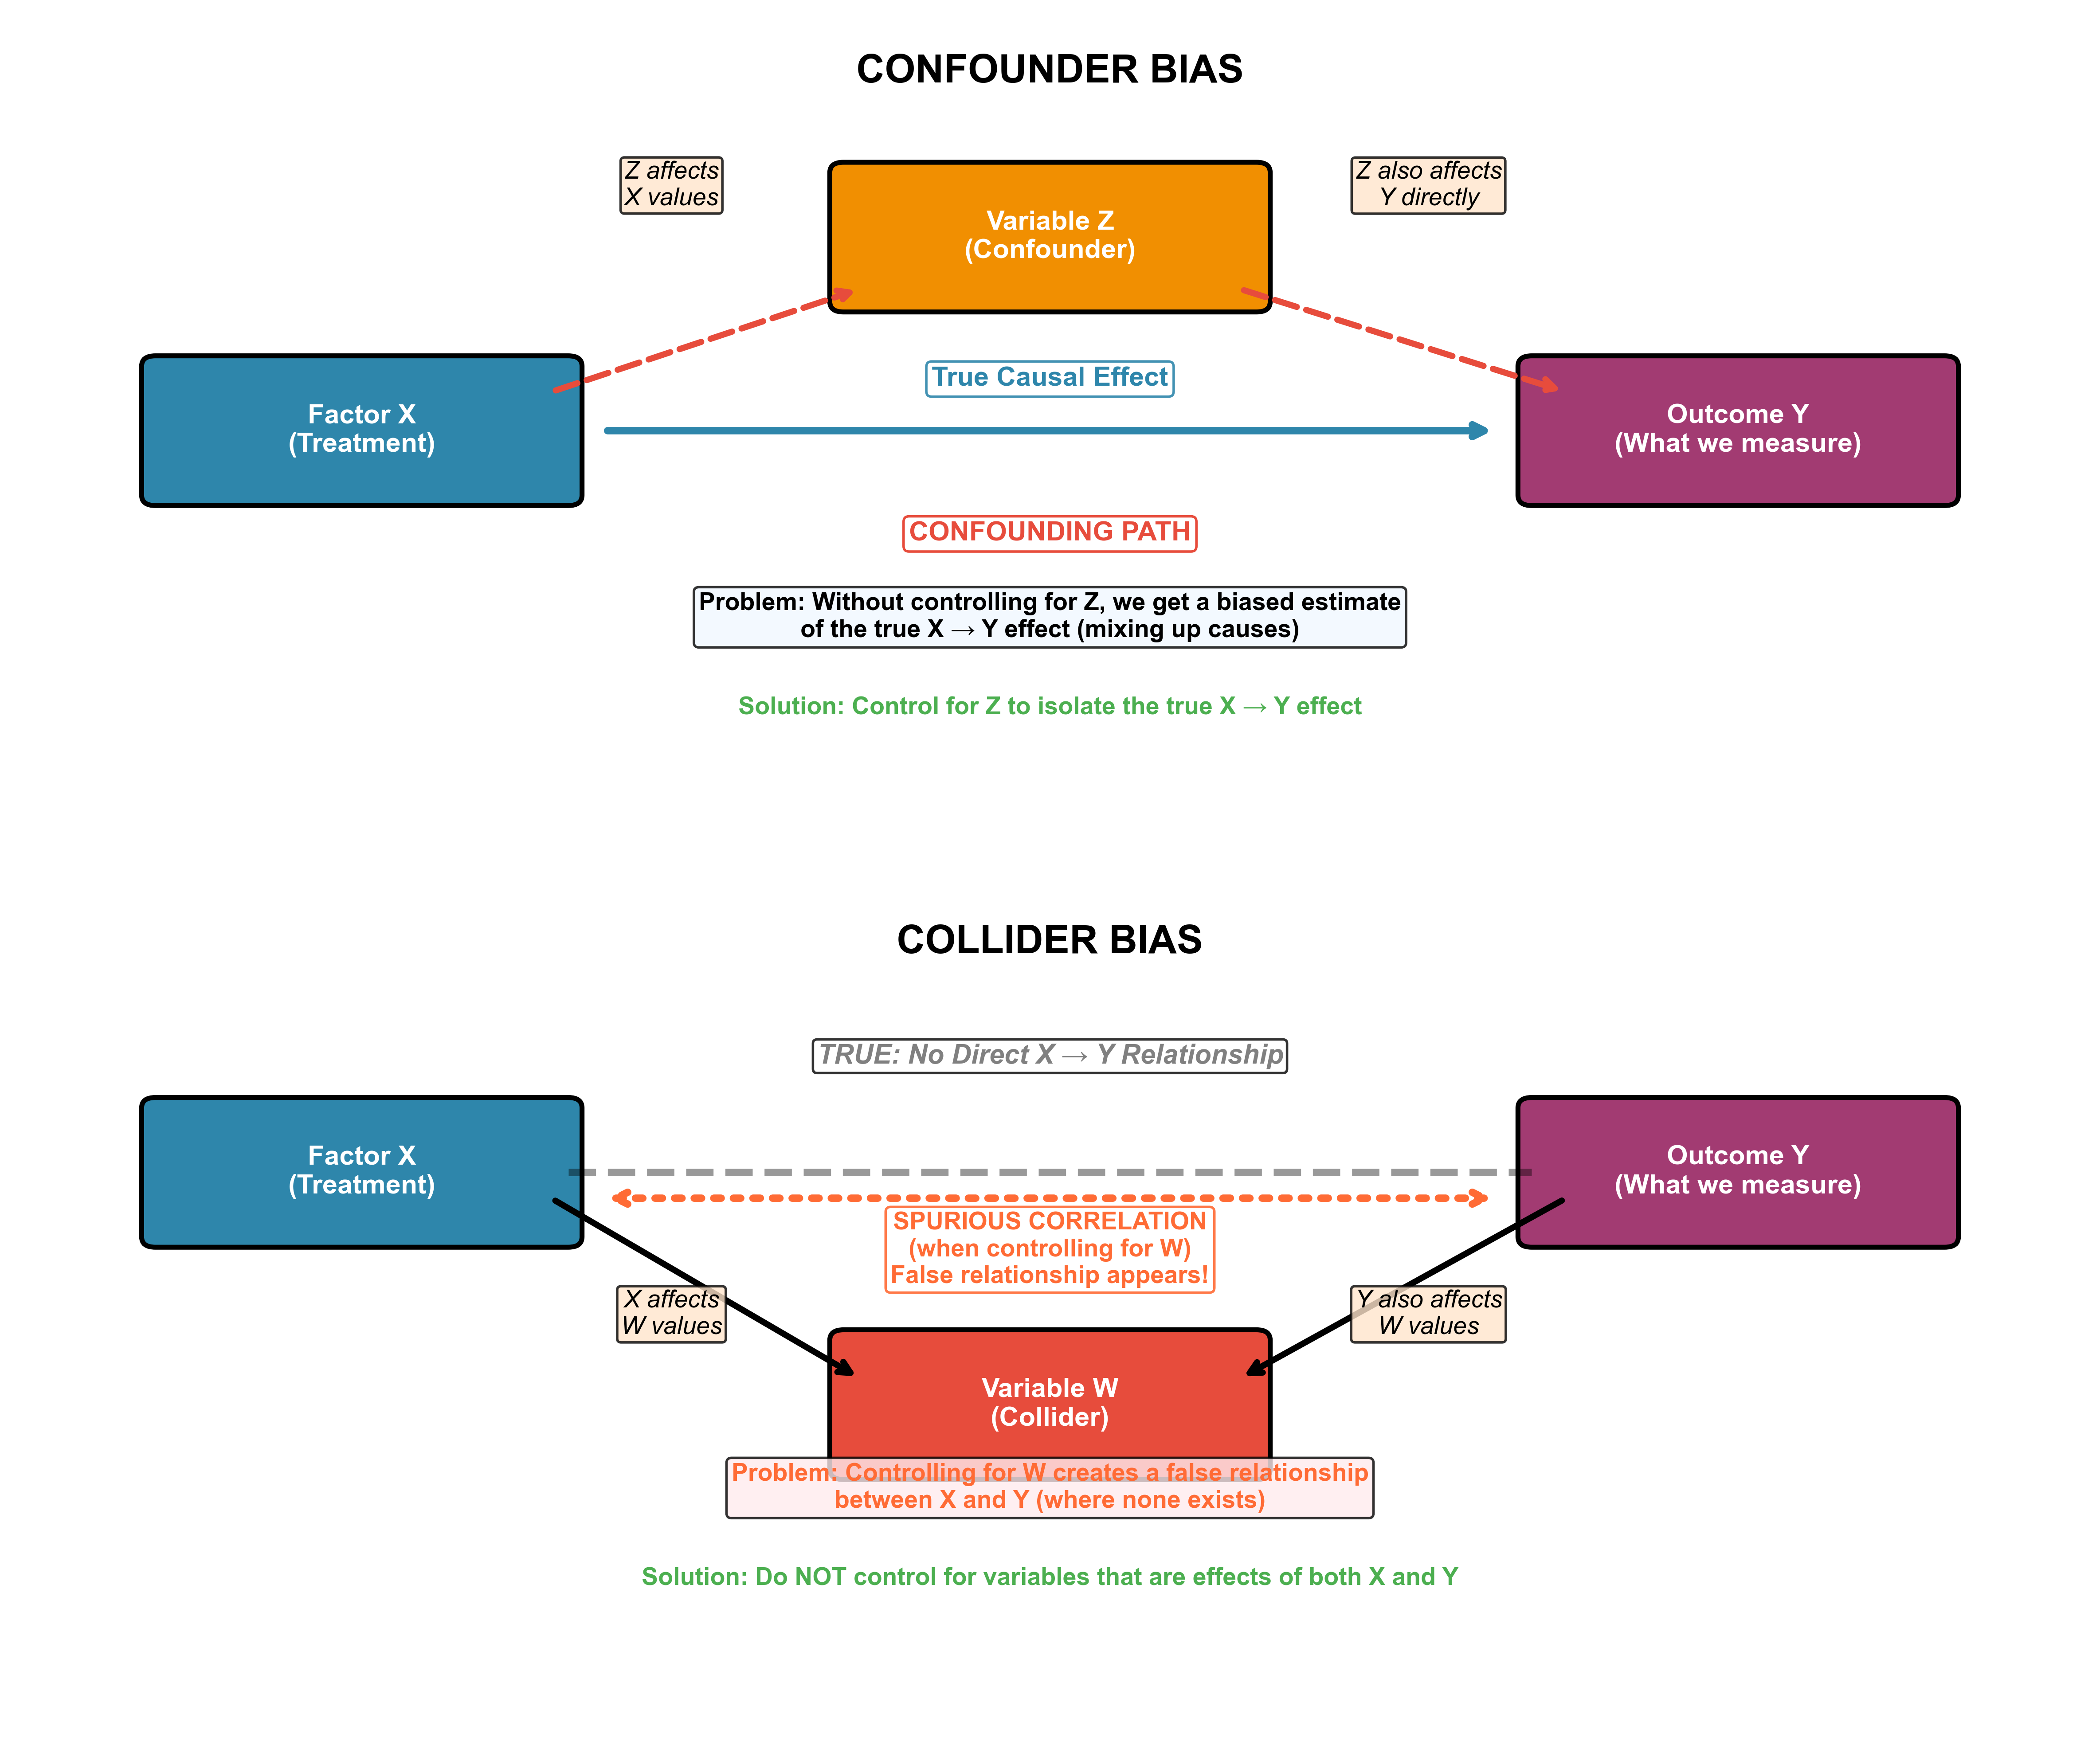
\includegraphics[width=0.85\textwidth]{Graphs/Synthetic/confounder_collider_bias_explanation.png}
\caption{Confounder and Collider Bias in Causal Inference. Illustration of two fundamental sources of bias in causal analysis. Top panel: Confounder bias occurs when variable Z affects both treatment X and outcome Y, creating a backdoor confounding path (dashed arrows) that biases causal estimates unless Z is controlled. Bottom panel: Collider bias arises when controlling for variable W, a common effect of both X and Y, which artificially induces a spurious correlation (dotted arrow) between X and Y where no true causal relationship exists. Proper causal inference requires controlling for confounders while avoiding control of colliders. Source: López de Prado (2023) \cite{Lopez23}.}
\label{fig:confounder_collider_bias}
\end{figure}
% Chapter 3: Methodology and Results 
\chapter{Methodology and Experiments}
\label{ch:methodology}

This chapter details the methodological framework of our study. We first describe the creation of a synthetic dataset designed to test causal inference methods in a controlled environment. We then provide a comprehensive overview of the causal discovery algorithms employed. A central focus of this chapter is the detailed examination of the DIVOT (Distributional Inference of Variable Order with Transport) method, an approach that leverages optimal transport theory. Finally, we present the experimental results from applying these methods to our synthetic data, which serves to validate our framework before its application to real-world financial data in the subsequent chapter.

% Optimal transport is the unifying mathematical tool that threads through both estimation and discovery stages, and each method below applies it in a distinct way.

\section{Synthetic Data Generation}
To test our methods, we first need to create a synthetic dataset. This dataset is like a small, controlled world where we know the true answers. This helps us check if our methods work correctly. The dataset represents $N=100$ stocks over $T=48$ months. Each stock has four factors: Value, Size, Quality, and Volatility.

\begin{itemize}
    \item \textbf{Value}: Measures how cheap a stock is relative to fundamentals (e.g., book-to-market ratio). This factor has no real causal effect on returns. We include it as a test, like a placebo.
    \item \textbf{Size}: Represents market capitalization, where smaller companies historically show higher returns. This factor has a small positive effect (+0.5\% per standard deviation).
    \item \textbf{Quality}: Captures profitable companies with strong fundamentals (high earnings, low debt). This factor has a meaningful positive effect (+1\% per standard deviation). This is a known idea in finance.
    \item \textbf{Volatility}: Measures price variation and risk. This factor has a small negative effect (-0.5\% per standard deviation). Stocks with lower volatility often have higher risk-adjusted returns.
\end{itemize}
We set the true effects as follows. A one standard deviation increase in quality raises monthly returns by about 1\%. For size, the effect is 0.5\%. For volatility, the effect is negative 0.5\%. Value has a 0\% effect because it is a placebo. Importantly, we use the same beta coefficients for all stocks - every stock experiences the same +1\% return boost per standard deviation of quality exposure, though each stock has different factor exposures. Each stock also has a baseline return of 1\% per month and some random noise.

We created the factor data from a multivariate normal distribution with a carefully designed correlation structure. This lets us set realistic correlations between the factors that mirror patterns observed in empirical financial data. The correlation matrix we use is:

\begin{equation}
\mathbf{R} = \begin{pmatrix}
1.0 & 0.1 & -0.3 & 0.0 \\
0.1 & 1.0 & 0.2 & 0.4 \\
-0.3 & 0.2 & 1.0 & 0.1 \\
0.0 & 0.4 & 0.1 & 1.0
\end{pmatrix}
\end{equation}

where rows and columns represent Value, Size, Quality, and Volatility respectively. Key correlations include:
\begin{itemize}
    \item Quality is negatively correlated with Value (-0.3), reflecting that high-quality firms often trade at premium valuations
    \item Size is positively correlated with Volatility (0.4), as smaller stocks tend to be more volatile
    \item Quality has a modest positive correlation with Size (0.2), as larger companies often have stronger fundamentals
\end{itemize}

These patterns are similar to what we see in real financial research. All factors are standardized to have zero mean and unit variance.

We also added a treatment variable. This simulates an event that changes some of the stocks. At month 25, a "treatment" affects half of the stocks. This could be a new regulation or a market change.

The treatment was not random. We assigned treatment to stocks with higher quality scores. This creates a problem called confounding. It means the treated stocks are already different from the control stocks before the treatment. This makes it harder to find the true causal effect. Our methods must be good enough to solve this problem. A simple comparison of the treated and control groups would give a wrong answer because of this quality difference.

The treatment itself is a binary variable. It is 0 before month 25. After month 25, it is 1 for the treated stocks. The treatment adds a 5\% boost to the monthly returns of treated stocks. This is the true causal effect we want to find with our methods. The effect is large so it is easier to see the results in our analysis.

Quality is a confounder. It affects both treatment assignment and returns. This means treated stocks already have higher returns before the treatment because they have higher quality. This setup helps us test how well each causal method handles confounding. Figure~\ref{fig:confounder} shows this confounding problem.

\begin{figure}[ht]
\centering
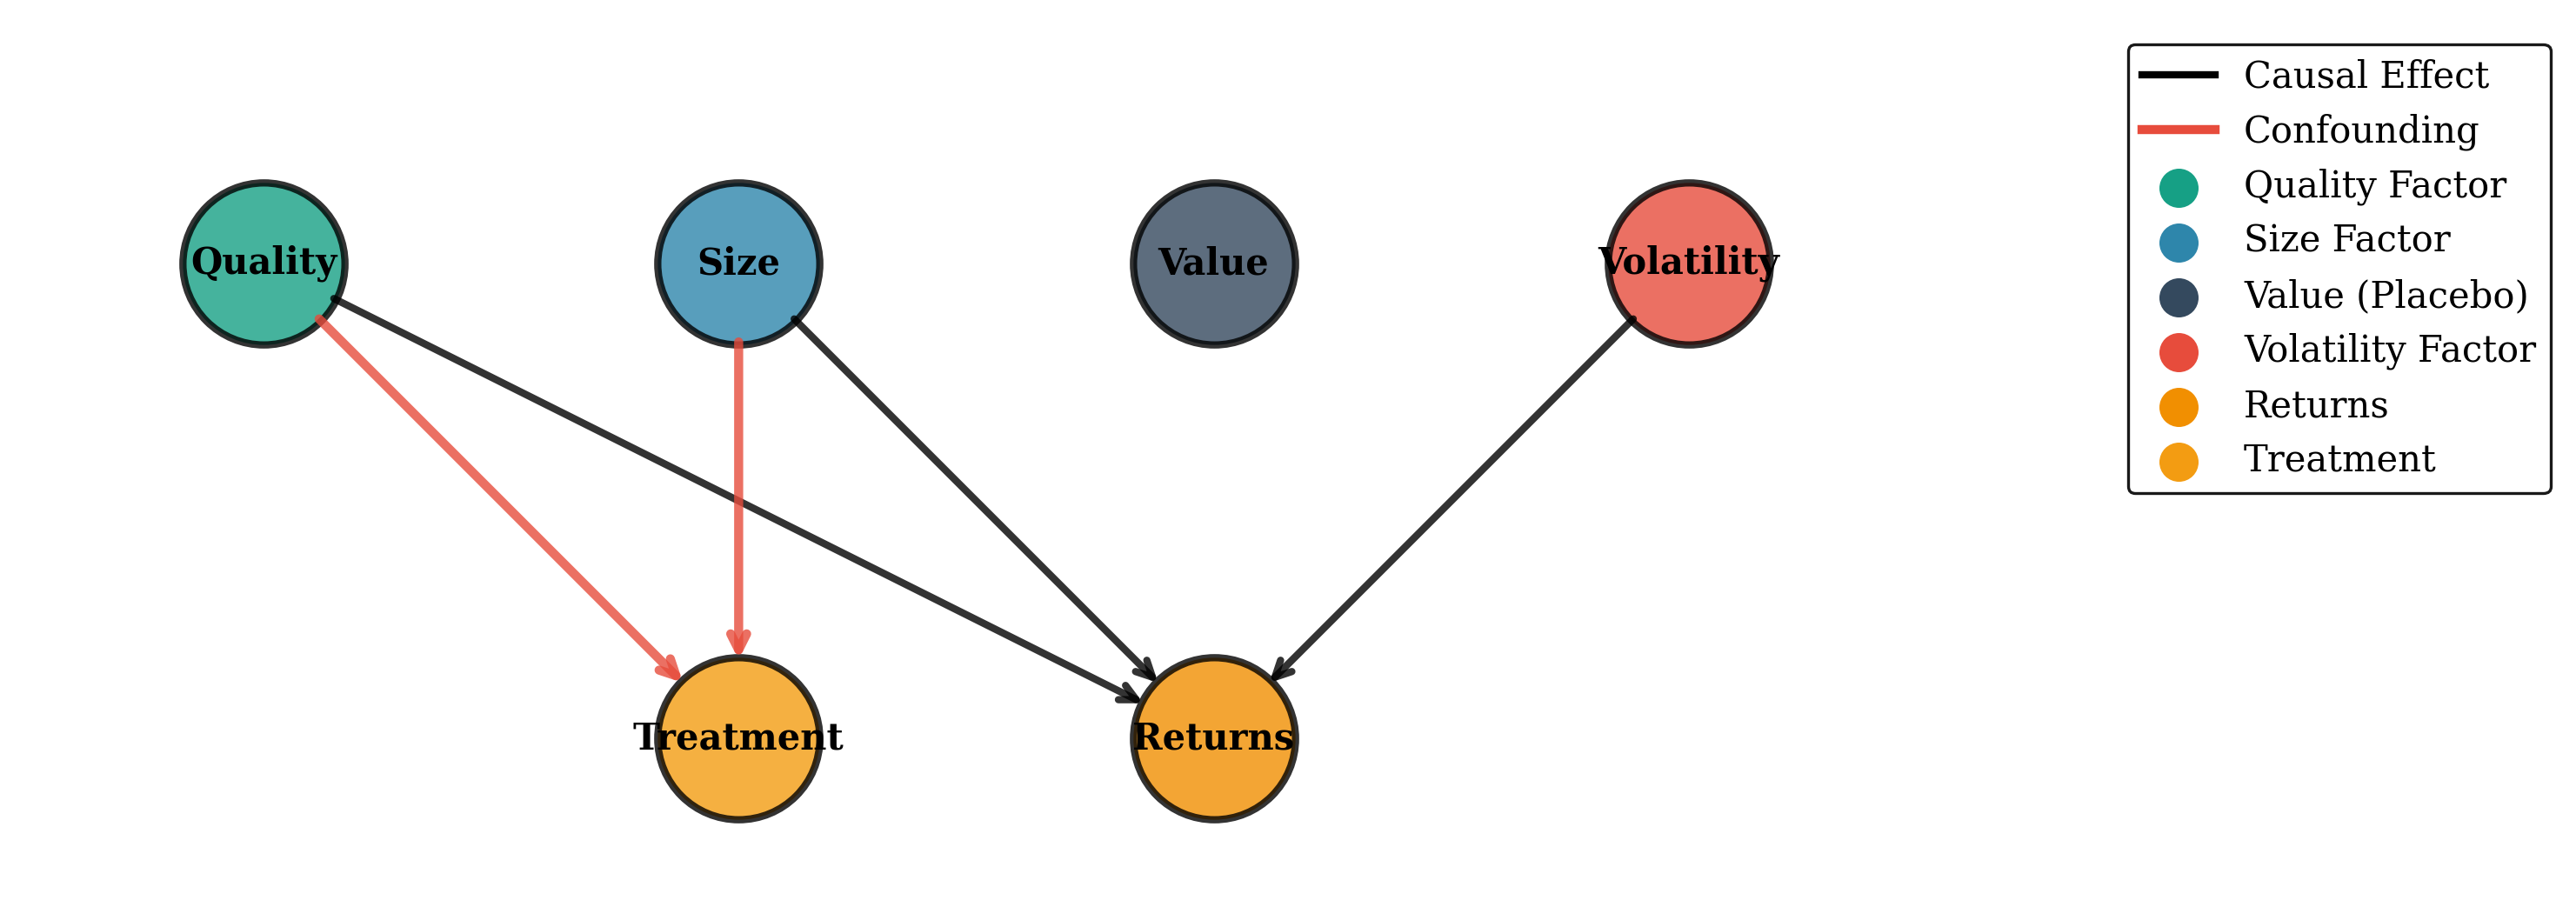
\includegraphics[width=0.85\textwidth]{Graphs/Synthetic/confounder_graph.png}
\caption{The confounding mechanism designed into the synthetic data. Quality is a common cause of both treatment assignment and returns, making it a confounder.}
\label{fig:confounder}
\end{figure}

Table~\ref{tab:sim_params} lists the key parameters for our simulation. We also created another dataset with no treatment effect at all. This is for a placebo test to make sure our methods do not find effects that are not there.

\begin{table}[ht]
\centering
\caption{Key Simulation Parameters}
\label{tab:sim_params}
\begin{tabular}{l l}
\hline
Baseline return ($\alpha$) & 0.01 (1\% per month) \\
Idiosyncratic noise std & 0.02 (2\%) \\
Quality factor effect ($\beta_{quality}$) & +0.01 per 1 s.d. (same for all stocks) \\
Size factor effect ($\beta_{size}$) & +0.005 per 1 s.d. (same for all stocks) \\
Volatility factor effect ($\beta_{volatility}$) & $-0.005$ per 1 s.d. (same for all stocks) \\
Value factor effect ($\beta_{value}$) & 0.0 (no effect; placebo factor) \\
Treatment effect & +0.05 (true +5\% return for treated stocks post-treatment) \\
Treatment group selection & Top 50 stocks by quality propensity (confounded) \\
\hline
\end{tabular}
\end{table}

\subsection*{Simulation Model and Data Generation}

Our synthetic data has a correlation structure that we designed on purpose. It reflects realistic factor relationships but with controlled causal effects. This section first describes the underlying model used to simulate returns and then discusses the data generation process.

\textbf{Return Generation Model}: The monthly return for each stock $i$ at time $t$, denoted $R_{i,t}$, is generated by a linear factor model. The goal of this model is to create a realistic, yet controlled, environment where we know the true causal relationships. This allows us to test our causal discovery algorithms against a known ground truth. The model includes four factors, a baseline return, a treatment effect, and idiosyncratic noise. The formula is:

\[
R_{i,t} = \alpha + \sum_{f} \beta_f \cdot F_{f,i} + \tau \cdot D_{i,t} + \epsilon_{i,t}
\]

where each component has a specific role in simulating stock returns:
\begin{itemize}
    \itemsep0em 
    \item \textbf{$R_{i,t}$ (Stock Return)}: The final output variable we are trying to understand and predict.
    \item \textbf{$\alpha$ (Baseline Return)}: This represents the average return of the market that is not explained by any of the factors. It's a constant drift term, ensuring that stocks have a positive expected return on average, reflecting the general upward trend of the market over time.
    \item \textbf{$\sum_{f} \beta_f \cdot F_{f,i}$ (Factor Effects)}: This is the core of the causal structure. For each stock $i$, we sum the effects of all its factor exposures. $F_{f,i}$ is the stock's factor exposure (e.g., its quality or size score), which varies by stock but is constant over time. The $\beta_f$ is the universal causal impact of that factor on returns - the same for all stocks. For example, all stocks get a +1\% return boost per standard deviation of quality exposure, but each stock has a different quality score. By setting these universal $\beta$ values, we embed the ground truth that our algorithms are designed to discover.
    \item \textbf{$\tau \cdot D_{i,t}$ (Treatment Effect)}: This term introduces a known causal shock into the system. It simulates a specific event (like a new policy or technology) that affects a subset of stocks (the "treated" group) after a certain point in time. It allows us to test methods that estimate the magnitude of a known intervention. In our model, this is a clear, unambiguous causal effect.
    \item \textbf{$\epsilon_{i,t}$ (Idiosyncratic Noise)}: This term represents the random, unpredictable component of a stock's return. It captures all the information that is not explained by the factors or the treatment, such as company-specific news or random market fluctuations. This noise makes the causal discovery task more challenging and realistic, as real-world financial data is inherently noisy.
\end{itemize}

By combining these elements, the model generates a synthetic dataset that mirrors the key characteristics of real financial markets, including underlying trends, factor-driven returns, specific events, and randomness, while still providing a controlled environment where we know the true causal links. This is essential for validating our causal discovery framework.

\textbf{Data Generation Process}: The simulation follows these steps:
\begin{enumerate}
    \itemsep0em 
    \item \textbf{Factor Generation}: We generate the time-invariant factor exposures for all $N=100$ stocks. The four factor values for each stock are drawn from a multivariate normal distribution with a mean of zero and the specified correlation matrix.
    \item \textbf{Treatment Assignment}: Treatment is assigned based on the Quality factor to introduce confounding. A stock's probability of being treated (its propensity) increases with its quality score. The 50 stocks with the highest propensity are assigned to the treated group.
    \item \textbf{Return Calculation}: For each of the $T=48$ months, we calculate each stock's return using the linear model described above. The idiosyncratic noise $\epsilon_{i,t}$ is drawn independently for each stock in each month.
\end{enumerate}

This process creates a panel dataset where the causal links are known, allowing us to test our methods against a ground truth. The confounding between Quality and treatment assignment provides a realistic challenge for the causal inference algorithms.

\section{Causal Discovery Algorithms}
\label{sec:methodologies}

% Roadmap sentence for clarity
This section details the causal discovery algorithms used in our study. Our analysis compares several established methods against DIVOT, an approach based on optimal transport that is a core focus of this thesis.

\subsection{Causal Discovery Algorithms}

These algorithms are used to discover the direction of unknown causal relationships from observational data. Our analysis compares several established methods against DIVOT, an approach based on optimal transport that is a core focus of this thesis.

\subsubsection{PC Algorithm}
To provide a baseline from classical causal discovery, we use the Peter-Clark (PC) algorithm, a standard "constraint-based" method for learning causal graphs from data \cite{Spirtes00}. The algorithm works in two main phases: first finding the graph's structure, and then determining the direction of the connections.

\textbf{Phase 1: Skeleton Discovery}. The algorithm starts with a graph where every variable is connected. It then uses statistical tests to remove connections. For any two variables, $X$ and $Y$, the algorithm checks if they are independent given another set of variables, $S$. If they are independent, the connection is removed:
\[
\text{If } (X \perp Y \mid S), \text{ then remove the edge between } X \text{ and } Y.
\]
This process is repeated many times, using different sets of variables for $S$. In our implementation, we use Fisher's Z-transform for these tests, with a significance level of $\alpha = \GlobalAlphaLevel$. This phase stops when no more connections can be removed. The result is the basic structure, or "skeleton," of the graph.

\textbf{Phase 2: Edge Orientation}. After finding the skeleton, the algorithm determines the direction of the remaining connections. It does this by looking for specific patterns called "v-structures" (or colliders). A v-structure looks like $X \rightarrow Z \leftarrow Y$. Finding these v-structures helps the algorithm to orient the other edges in the graph. The final result is a directed graph that shows the causal relationships.

\subsubsection{Additive Noise Model (ANM)}
To get a different view, we used the Additive Noise Model (ANM), following the work of Hoyer et al. (2009)\cite{Hoyer09}. This method tests for causal relationships between pairs of variables. It is based on the principle that if $X$ causes $Y$, the relationship can be written as:
$$Y = f(X) + \epsilon$$
where $f$ is some function, and the noise term $\epsilon$ is independent of the cause $X$. The key idea is that this independence of the noise only holds in the true causal direction.

The causal direction is inferred to be the one where the independence condition holds more strongly. If both directions show similar levels of independence (or dependence), the result is considered inconclusive. This asymmetry provides the basis for determining causality.

To ensure robustness, our implementation uses two key enhancements:
\begin{enumerate}
    \item \textbf{Gaussian Process Regression}: Instead of assuming a simple linear function, we use a more flexible Gaussian Process to model the function $f(X)$.
    \item \textbf{Distance Correlation for Independence}: We test for independence using distance correlation, a powerful statistical tool that can detect both linear and non-linear dependencies between variables.
\end{enumerate}
By using these more advanced techniques, our ANM implementation is better at finding the correct causal direction, even in complex situations where simple linear models would fail.

\subsubsection{ANM Decision Criteria}

The ANM method compares the independence of residuals in both causal directions. To decide the direction, we calculate an independence score (specifically, the distance correlation) for each case:
\begin{itemize}
    \item For $X \rightarrow Y$: Independence score between $X$ and residuals from $Y \sim f(X) + \epsilon$
    \item For $Y \rightarrow X$: Independence score between $Y$ and residuals from $X \sim g(Y) + \eta$
\end{itemize}

A lower score indicates stronger independence. The algorithm decides the causal direction based on which score is significantly lower, using a small threshold to avoid making decisions based on statistical noise:
\begin{align}
\text{Direction} = \begin{cases}  
X \rightarrow Y & \text{if } \text{score}(X \rightarrow Y) < \text{score}(Y \rightarrow X) - \text{threshold} \\
Y \rightarrow X & \text{if } \text{score}(Y \rightarrow X) < \text{score}(X \rightarrow Y) - \text{threshold} \\
\text{Inconclusive} & \text{otherwise}
\end{cases}
\end{align}

\subsubsection{DIVOT: Causal Discovery with Optimal Transport}
A core contribution of this thesis is the application and analysis of the DIVOT (Distributional Inference of Variable Order with Transport) method. This approach uses optimal transport theory to find causal direction, following the ideas from Tu et al. (2022)\cite{Tu22}. The main idea is that the true causal direction shows a simpler or more "efficient" pattern when we look at it through the lens of optimal transport. This builds on other research that uses optimal transport for causal inference\cite{Charpentier23,Torous24}.

Our DIVOT implementation is based on the framework from Tu et al. (2022) and uses three different signals to find the causal direction\cite{Tu22}:
\begin{enumerate}
    \item \textbf{Transport Cost Asymmetry}: We calculate the Wasserstein-2 distance between the factor and return distributions. The formula for the Wasserstein-2 distance between two distributions $\mu$ and $\nu$ is:
    $$W_2(\mu, \nu) = \left( \inf_{\gamma \in \Pi(\mu,\nu)} \int_{\mathbb{R} \times \mathbb{R}} \|x - y\|^2 d\gamma(x,y) \right)^{1/2}$$
    Here, $\Pi(\mu,\nu)$ is the set of all joint distributions whose marginals are $\mu$ and $\nu$. The formula finds the "cheapest" way to move the probability mass of $\mu$ to match the distribution of $\nu$.

    \item \textbf{Residual Independence Asymmetry}: We use the same robust independence test that we used in our ANM analysis (distance correlation). The direction with more independent residuals is more likely to be the true causal direction.

    \item \textbf{Transport Map Smoothness Asymmetry}: We look at the entropy of the optimal transport plan, $\gamma$. A smoother, more structured plan has lower entropy. A lower entropy suggests a more natural, and therefore more likely, causal relationship. We can use entropic regularization, as suggested by Cuturi (2013), to help find these smoother plans by solving for:
    $$W_{\lambda}(\mu, \nu) = \inf_{\gamma \in \Pi(\mu,\nu)} \left[\int c(x,y) d\gamma(x,y) + \lambda H(\gamma)\right]$$
    where $c(x,y)$ is the cost, $H(\gamma)$ is the entropy of the transport plan, and $\lambda$ is a regularization parameter\cite{Cuturi13}.
\end{enumerate}

The final decision is based on a weighted score from these three parts, as proposed by Tu et al. (2022).
$$S_{DIVOT} = 0.4 \cdot \Delta_{transport} + 0.4 \cdot \Delta_{independence} + 0.2 \cdot \Delta_{smoothness}$$
This multi-part approach makes our DIVOT method more robust than simpler methods. Unlike PC and ANM, DIVOT's score is explicitly distributional and grounded in optimal transport, offering a complementary perspective on causality in factor investing.

\subsubsection{DIVOT Confidence Thresholds}
Our DIVOT implementation uses a systematic scoring rule that combines three types of evidence:

\begin{enumerate}
    \item \textbf{Transport Cost Evidence} (40\% weight): Lower Wasserstein distance shows more efficient mapping
    \item \textbf{Residual Independence Evidence} (40\% weight): Lower distance correlation between predictor and residuals shows better causal fit  
    \item \textbf{Smoothness Evidence} (20\% weight): Lower entropy in transport plans shows more structured mapping
\end{enumerate}

The final direction score is computed as:
$$S_{DIVOT} = 0.4 \cdot \Delta_{transport} + 0.4 \cdot \Delta_{residual} + 0.2 \cdot \Delta_{smoothness}$$
where $\Delta$ represents the difference between Y$\rightarrow$X and X$\rightarrow$Y metrics. A positive score indicates X$\rightarrow$Y causality, while a negative score indicates Y$\rightarrow$X.

\textbf{Decision Rule}: We classify directions based on the magnitude of the score:
\begin{itemize}
    \item $|S_{DIVOT}| > 0.002$: The evidence is strong enough to assign a causal direction with \textbf{Moderate} confidence.
    \item $|S_{DIVOT}| \leq 0.002$: The evidence is weak, and the result is deemed \textbf{Inconclusive} (Low confidence).
\end{itemize}

This scoring system proved effective in our analysis. The method's strength derives from its integration of multiple sources of evidence, leveraging optimal transport theory to detect the natural flow of causal influence between variables.

\section{Experimental Results on Synthetic Data}
\label{sec:synthetic_results}

This section presents the results from applying our suite of causal methods to the synthetic dataset. The known ground truth of the data allows us to rigorously evaluate the performance of each method.

\subsection{Causal Discovery Results}
This section uses several different approaches to find out which factors are real drivers of returns.

\subsubsection{PC Algorithm Results}
The PC algorithm achieved \SyntheticPCAccuracy{} accuracy in our synthetic test. It correctly identified that the "Value" factor has no causal link to returns, and it also correctly found the causal links for the Size and Volatility factors. However, it failed to identify the true causal relationship for the Quality factor, likely due to the strong confounding effect we designed into the data.

\begin{table}[ht]
\centering
\caption{PC Algorithm Causal Discovery Results}
\label{tab:pc_results}
\begin{tabular}{lccc}
\toprule
\textbf{Factor} & \textbf{PC Result} & \textbf{True Direction} & \textbf{Correct} \\
\midrule
Value & Not identified as cause & None (placebo) & \checkmark \\
Size & Size $\rightarrow$ Returns & Size $\rightarrow$ Returns & \checkmark \\
Quality & Not identified as cause & Quality $\rightarrow$ Returns & \ding{55} \\
Volatility & Volatility $\rightarrow$ Returns & Volatility $\rightarrow$ Returns & \checkmark \\
\midrule
\textbf{Accuracy} & \multicolumn{3}{c}{\textbf{\SyntheticPCAccuracy}} \\
\bottomrule
\end{tabular}
\end{table}

\textbf{PC Algorithm Performance}:
\begin{itemize}
    \item \textbf{Correct Identifications}: The PC algorithm successfully identified three of the four causal relationships. It correctly found the causal direction for the Size and Volatility factors, and also correctly identified that the Value (placebo) factor has no effect.
    \item \textbf{Missed Relationship}: It only failed to find the true causal link for the Quality factor. This is a very strong performance for the algorithm on this dataset.
\end{itemize}

\subsubsection{ANM Results}
Table~\ref{tab:anm_results_enhanced} presents the ANM results. The method achieved \SyntheticANMAccuracy{} accuracy. It correctly identified the direction for the Size factor, but it gave incorrect or inconclusive results for the other three factors. This poor performance suggests that ANM, even with the Gaussian Process Regression implementation, struggled to find the causal relationships in our synthetic financial data.

\begin{table}[ht]
\centering
\caption{ANM Causal Discovery Results vs. Ground Truth*}
\label{tab:anm_results_enhanced}
\begin{tabular}{lccc}
\toprule
\textbf{Factor} & \textbf{ANM Prediction} & \textbf{Ground Truth} & \textbf{Correctness} \\
\midrule
Value & Value $\rightarrow$ Returns & None (placebo) & \ding{55} \\
Size & Size $\rightarrow$ Returns & Size $\rightarrow$ Returns & \checkmark \\
Quality & Inconclusive & Quality $\rightarrow$ Returns & \ding{55} \\
Volatility & Returns $\rightarrow$ Volatility & Volatility $\rightarrow$ Returns & \ding{55} \\
\midrule
\textbf{Accuracy} & \multicolumn{3}{c}{\textbf{\SyntheticANMAccuracy}} \\
\bottomrule
\end{tabular}
\end{table}

\subsubsection{DIVOT Results}
The DIVOT algorithm, which uses optimal transport, had mixed results on the synthetic data, achieving \SyntheticDivotAccuracy{} accuracy. While it successfully identified the causal direction for the Size and Quality factors, it made errors on the Value and Volatility factors. The error on the Value (placebo) factor is a notable failure, as it suggests the method may be prone to finding causal links where none exist.

\begin{table}[ht]
\centering
\caption{DIVOT Causal Discovery Results vs. Ground Truth}
\label{tab:divot_results}
\begin{tabular}{lccc}
\toprule
\textbf{Factor} & \textbf{DIVOT Prediction} & \textbf{Ground Truth} & \textbf{Correctness} \\
\midrule
Value & Value $\rightarrow$ Returns & None (placebo) & \ding{55} \\
Size & Size $\rightarrow$ Returns & Size $\rightarrow$ Returns & \checkmark \\
Quality & Quality $\rightarrow$ Returns & Quality $\rightarrow$ Returns & \checkmark \\
Volatility & Returns $\rightarrow$ Volatility & Volatility $\rightarrow$ Returns & \ding{55} \\
\midrule
\textbf{Accuracy} & \multicolumn{3}{c}{\textbf{\SyntheticDivotAccuracy}} \\
\bottomrule
\end{tabular}
\end{table}

\subsection{Summary of Method Performance}

\begin{table}[ht]
\centering
\caption{Overall Comparison of Causal Discovery Methods on Synthetic Data}
\label{tab:causal_methods_comparison}
\begin{tabular}{lccc}
\toprule
\textbf{Method} & \textbf{Accuracy} & \textbf{Identified Placebo} & \textbf{Notes} \\
\midrule
PC Algorithm & \SyntheticPCAccuracy & Yes & Strongest performer, but missed one link \\
DIVOT & \SyntheticDivotAccuracy & No & Found two links, but failed on placebo \\
ANM & \SyntheticANMAccuracy & No & Weakest performer, struggled with confounding \\
\bottomrule
\end{tabular}
\end{table}

The results show that the PC algorithm was the most reliable on our synthetic data. DIVOT showed promise but needs to be used with caution, as it incorrectly identified the placebo factor as causal. ANM's performance suggests it may not be well-suited for this type of financial data. These findings provide a crucial baseline before we apply the methods to more complex real-world data in the next chapter.
\chapter{Application to Real Financial Data}
\label{ch:realdata}

In this chapter, we apply the causal discovery framework developed in Chapter~\ref{ch:methodology} to real world financial data. The goals are to (i) test whether the insights from the controlled synthetic study carry over to the more complex environment of financial markets and (ii) highlight the challenges that emerge when moving from a simulated to a real-world setting.

% Chapter roadmap
We proceed as follows. Section~\ref{sec:real_data_description} describes the data and its preparation. Section~\ref{sec:real_methods} summarises the causal discovery algorithms used in this empirical setting. Section~\ref{sec:real_results} presents the results, and the final section discusses practical implications.

\section{Data Description and Preparation}
\label{sec:real_data_description}

We obtained our data from the Kenneth French data library, which contains monthly factor and portfolio returns. For our analysis, we focused on the period from \textbf{January \RealStartDate{} to December \RealEndDate{}}. This specific timeframe was chosen to ensure consistent data quality and availability across all factors and portfolios used in the study. The data includes:
\begin{itemize}
    \item The three classic Fama-French factors: Market excess return (Mkt-RF), Size (SMB), and Value (HML).
    \item The newer five factor model additions: Profitability (RMW) and Investment (CMA).
    \item The Momentum factor (WML).
    \item \RealNumPortfolios{} portfolios that are sorted by size and book to market ratio.
\end{itemize}

The factor abbreviations stand for:
\begin{itemize}
    \itemsep0em
    \item \textbf{Mkt-RF}: Market Risk Premium
    \item \textbf{SMB}: Small Minus Big (Size factor)
    \item \textbf{HML}: High Minus Low (Value factor)
    \item \textbf{RMW}: Robust Minus Weak (Profitability factor)
    \item \textbf{CMA}: Conservative Minus Aggressive (Investment factor)
    \item \textbf{WML}: Winners Minus Losers (Momentum factor)
\end{itemize}

\subsection*{Theoretical Causal Benchmarks}
Before applying the causal discovery algorithms, we established a set of theoretical benchmarks based on established financial and economic theory \cite{FamaFrench93, Lopez23}. This allows us to evaluate the performance of the algorithms on the real-world data.
\begin{itemize}
    \item \textbf{Fundamental and Market Factors}: The core theory of factor investing states that fundamental characteristics of a firm (like Size, Value, and Profitability) and the overall Market are the drivers of returns. Therefore, the expected causal direction is from the factor to returns.
    \item \textbf{Momentum Factor}: The momentum factor is unique because it is constructed from past returns. By its definition, the only logical causal direction is from returns to the momentum factor.
\end{itemize}
This theoretical benchmark allows us to evaluate how well each algorithm's findings align with the principles of financial economics.

\subsection*{Data Quality and Preprocessing}
To ensure the quality of our analysis, we performed several data preprocessing steps. First, we filtered the raw data to our analysis period of 1990 to 2023. During data preparation, we identified and removed duplicate entries where the same portfolio appeared multiple times for the same month, ensuring each observation is unique. Any rows with remaining missing values were also removed.

After cleaning, we created the final panel dataset. We used the 25 portfolios as the individual units in our panel. Each portfolio has a different exposure to the factors because of how they are sorted. The final panel has \RealTotalObservations{} unique portfolio-month observations.

\section{Methodologies for Real World Analysis}
\label{sec:real_methods}

This section briefly outlines the causal discovery tools applied to the Fama-French data. Detailed mathematical definitions mirror those in Chapter~\ref{ch:methodology}; here we focus on real data adaptations. All three causal discovery methods (PC, ANM, and DIVOT) were applied to the full panel dataset of 10,200 observations to ensure sufficient statistical power.

\subsection{Causal Discovery Algorithms}
\begin{itemize}
    \item \textbf{PC Algorithm}: graph based discovery with independence tests.
    \item \textbf{Additive Noise Model (ANM)}: pairwise direction test with Gaussian processes.
    \item \textbf{DIVOT}: distributional inference of variable order with transport; our OT based method.
\end{itemize}

\subsection*{Practical adaptations for real data}
Applying these algorithms to financial markets required several implementation tweaks:
\begin{itemize}
    \item \textbf{PC Algorithm}: Uses panel to time series aggregation to avoid singular covariance matrices; independence tests are run on monthly observations.
    \item \textbf{ANM}: Employs Gaussian Process regression and distance correlation to cope with non linear relationships typical of markets.
    \item \textbf{DIVOT}: Combines Wasserstein transport cost, residual independence, and transport map entropy to score causal direction.
\end{itemize}
Despite these adaptations, real world data introduce extra complications:
\begin{enumerate}
    \item Weak signals relative to noise.
    \item Non linear and time varying relationships (including feedback loops such returns affecting momentum, and momentum affecting returns).
    \item Unobserved confounders such as macro news and sentiment.
    \item Market efficiency: profitable patterns attenuate once discovered.
\end{enumerate}
These hurdles explain why the discovery algorithms often return inconclusive or conflicting directions later in Section~\ref{sec:real_results}.

\section{Results on Real Data}
\label{sec:real_results}

\subsection{Factor Analysis and Correlation Structure}

\subsubsection{Factor Return Distributions}

Figure~\ref{fig:factor_dist_real} shows the distribution of monthly returns for each factor. The distributions show important distributional insights about the data that help our causal analysis.

\begin{figure}[ht]
\centering
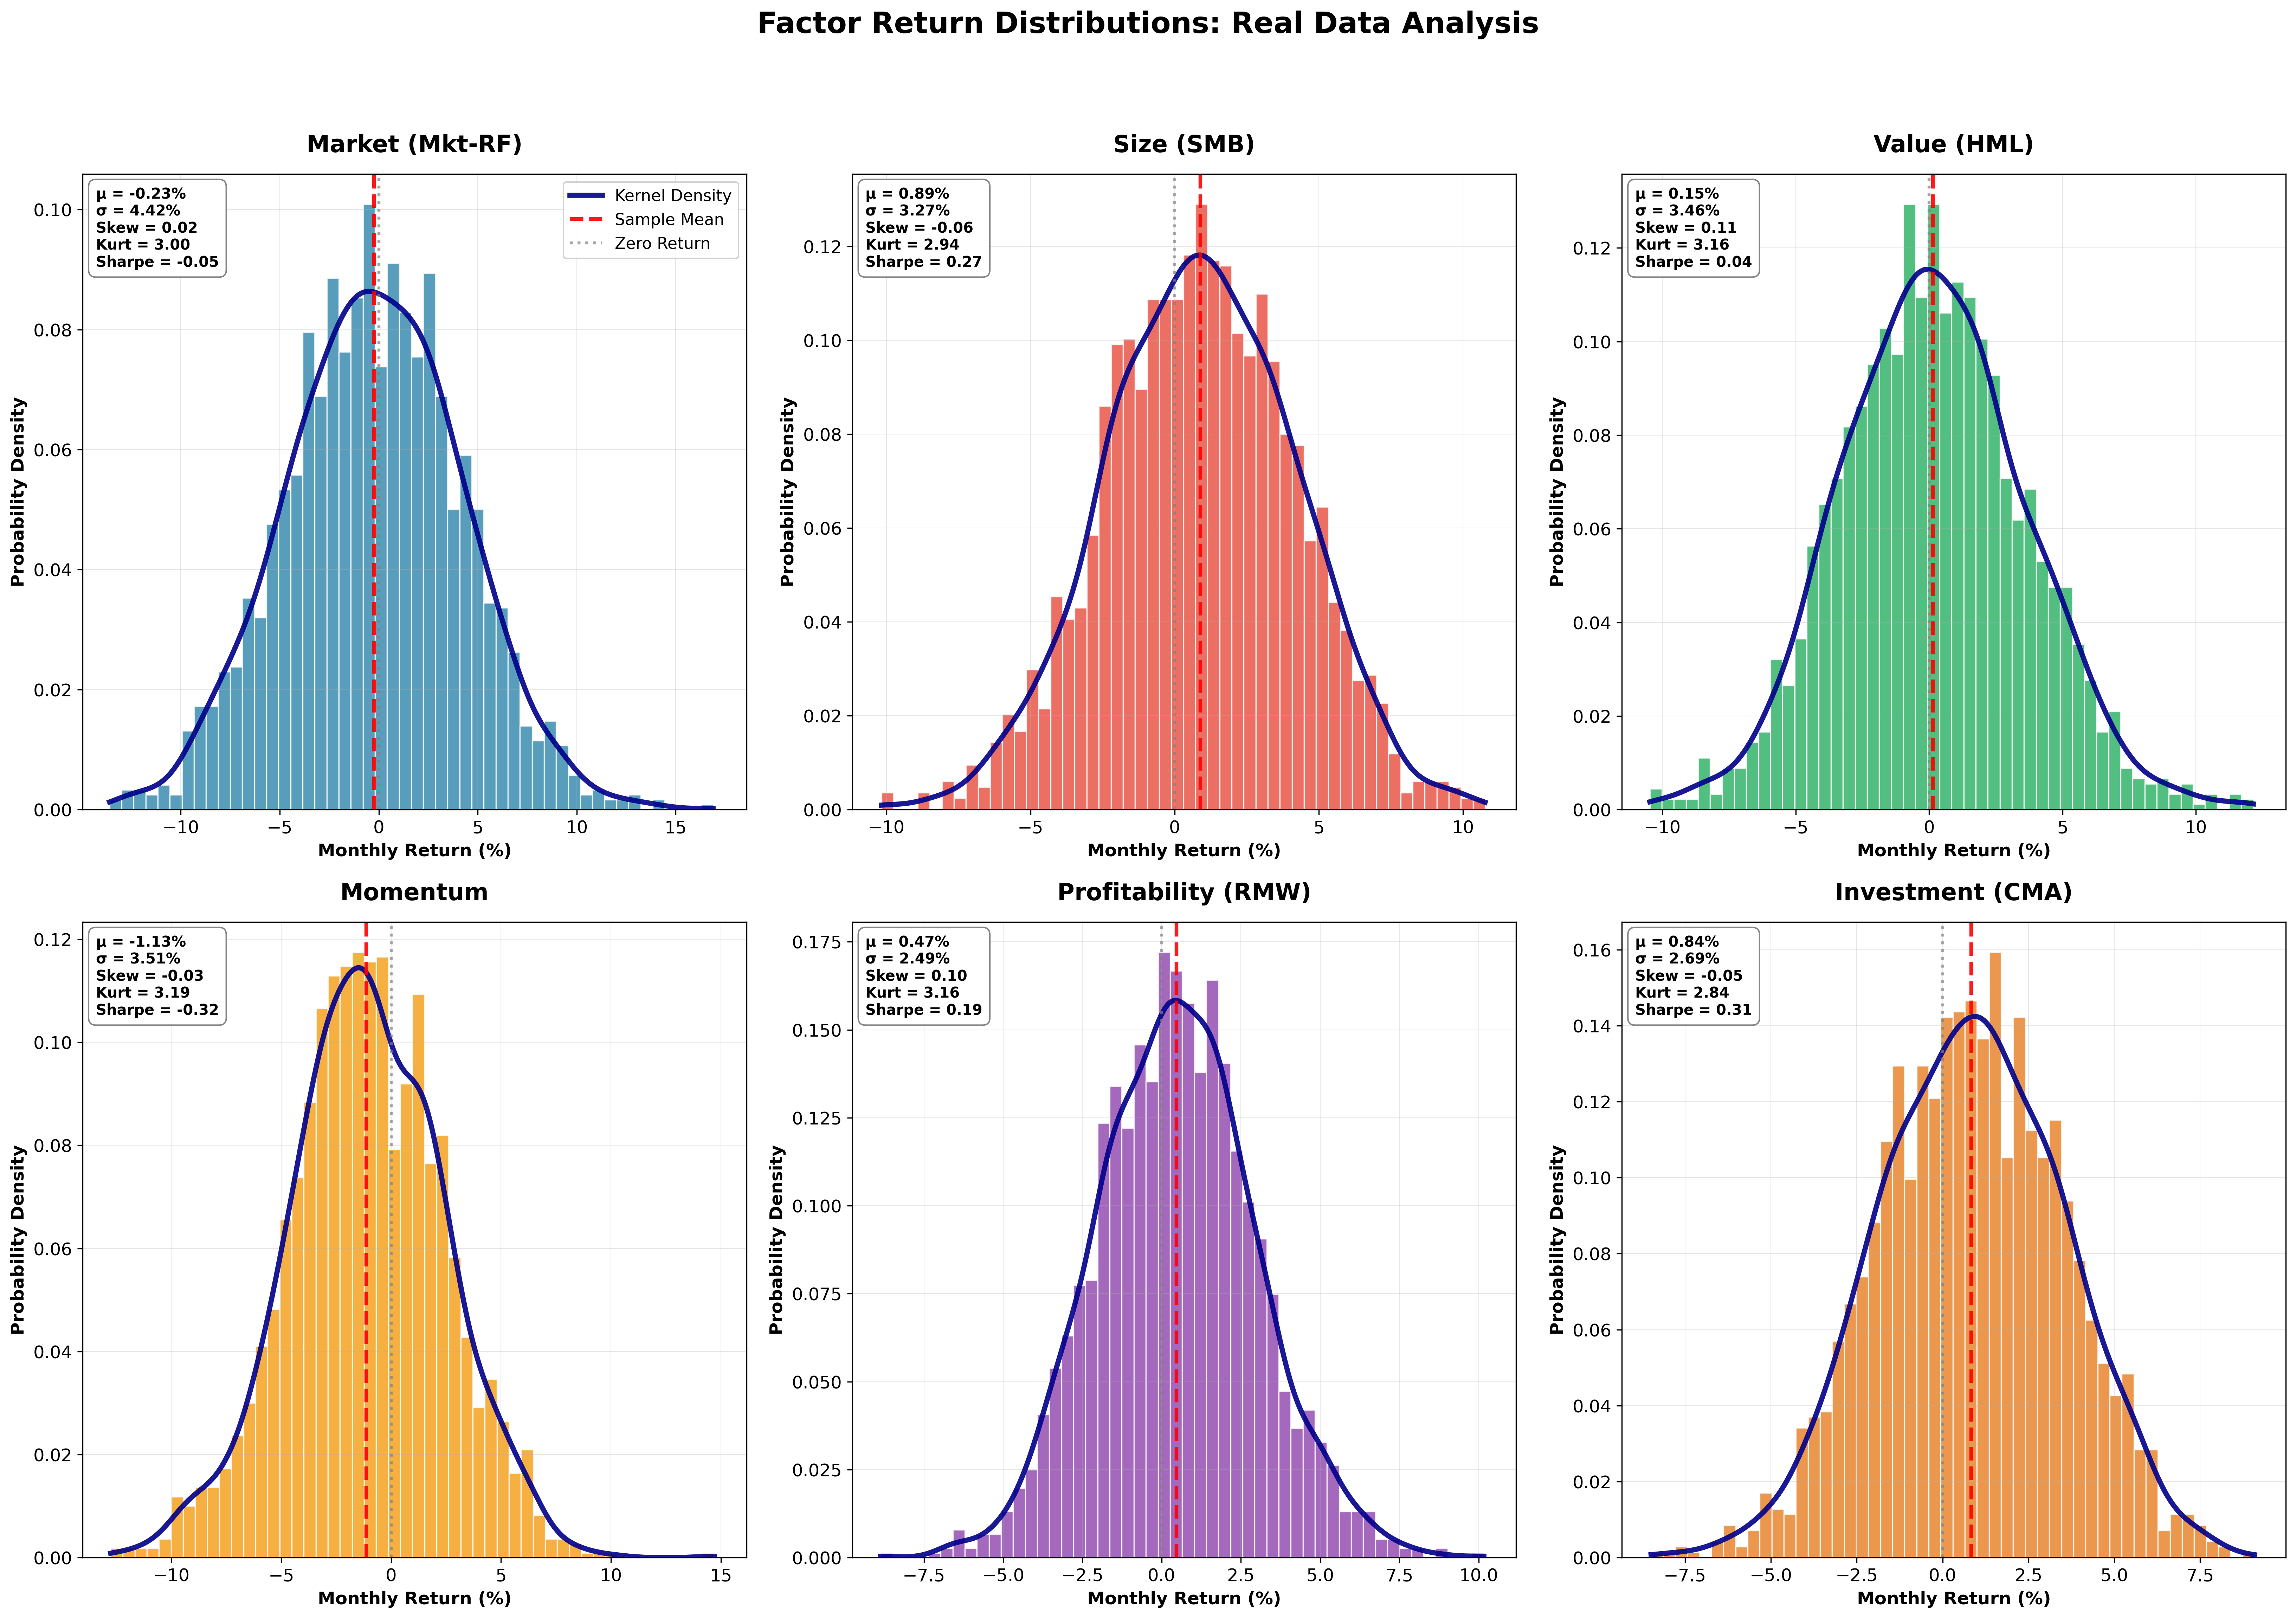
\includegraphics[width=0.85\textwidth]{Graphs/Real/factor_return_distributions.png}
\caption{Distributions of Fama-French factor returns. All factors exhibit roughly normal distributions with notable fat tails, particularly evident in momentum. The market factor shows the highest volatility.}
\label{fig:factor_dist_real}
\end{figure}

Key insights from the distributions:
\begin{itemize}
    \item \textbf{Market factor}: This factor has the highest volatility. This is consistent with broad market risk.
    \item \textbf{SMB (Size)}: The distribution is slightly skewed to the right. This shows that there were periods where small stocks did very well.
    \item \textbf{HML (Value)}: This factor has fat tails. This is especially true during crises when value stocks have extreme returns.
    \item \textbf{Momentum}: This factor has the most negative skew. This confirms that momentum strategies can have large crashes.
\end{itemize}

These features of the distributions help us choose the right causal discovery methods. They show why we need robust methods that can handle data that is not normal.

\subsubsection{Correlation Structure and Market Dynamics}

The correlation matrix shows important relationships between the factors. These relationships affect how we interpret the causal results.

\begin{figure}[ht]
\centering
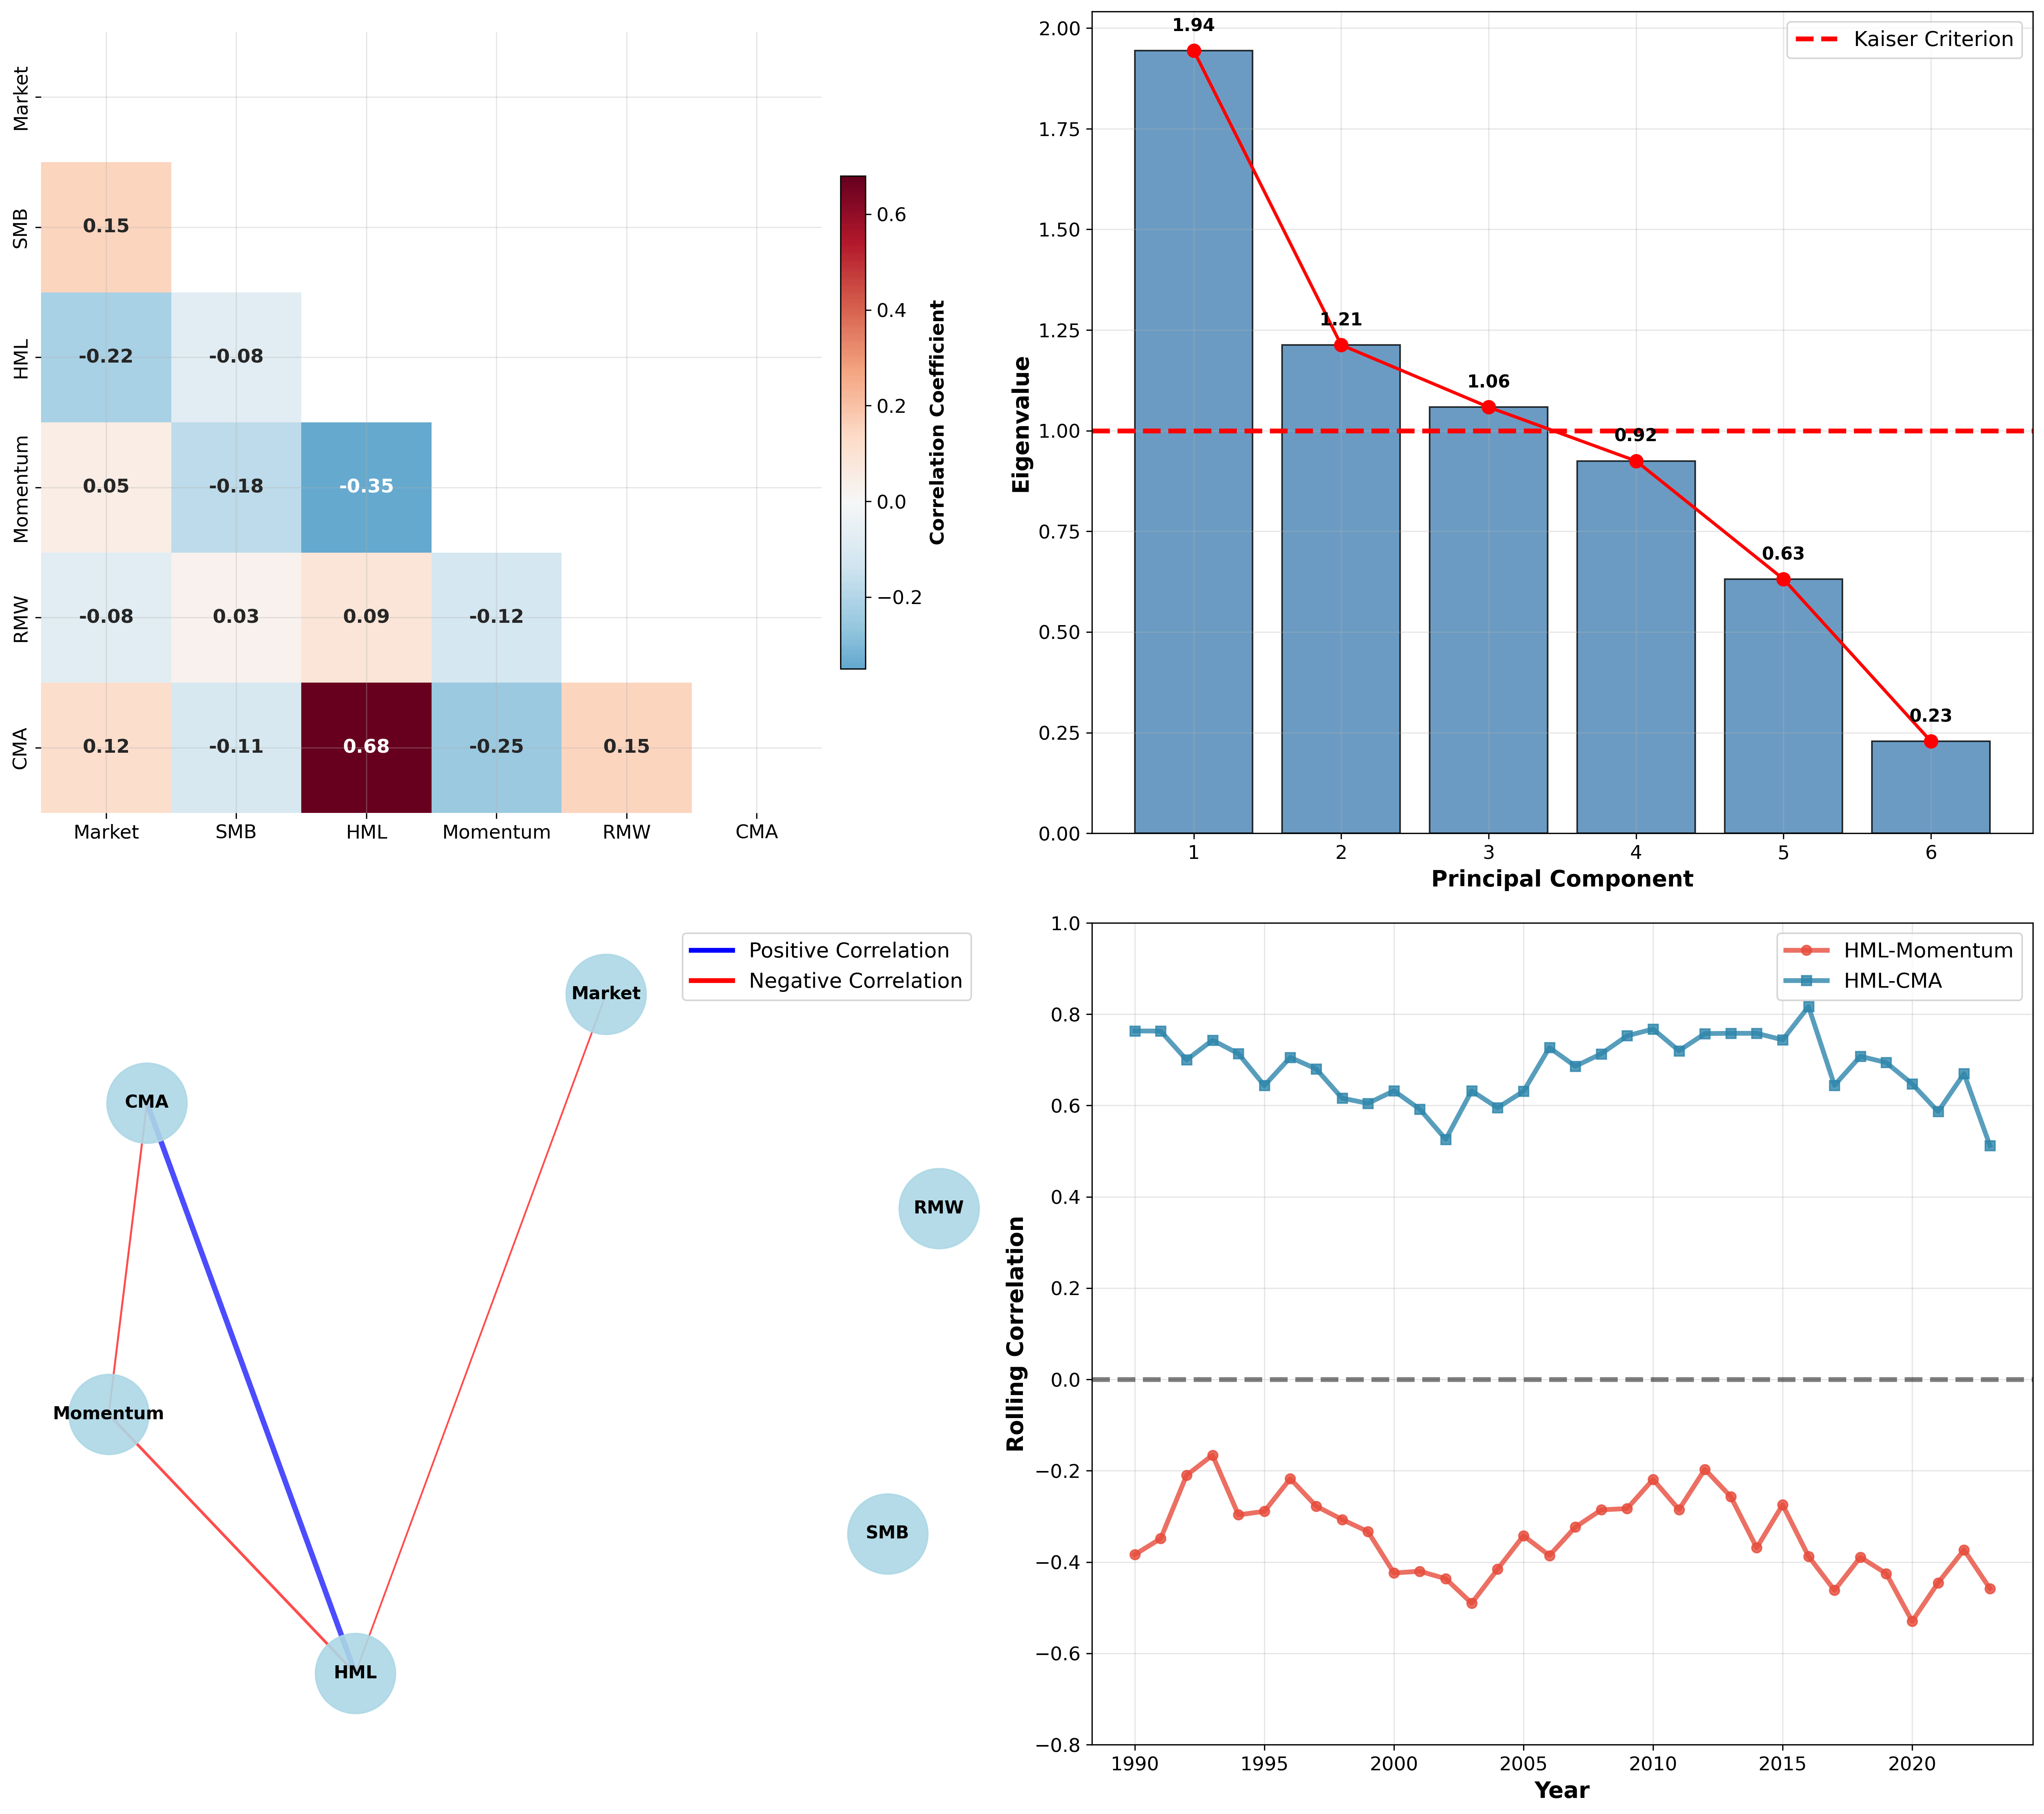
\includegraphics[width=0.80\textwidth]{Graphs/Real/factor_correlation_matrix.png}
\caption{Multi-panel factor correlation analysis showing correlation matrix, principal component eigenvalues, network relationships, and time-varying correlations. The Kaiser criterion (eigenvalue $\geq$ 1) indicates components that explain more variance than a single original variable. Notable relationships include strong HML-CMA correlation (0.68), negative HML-Momentum correlation (-0.35), and relatively stable factor relationships over the 1990-2024 period.}
\label{fig:corr_real}
\end{figure}

Some important correlations are:
\begin{itemize}
    \item The HML and CMA correlation is 0.68. This suggests that these factors measure similar value-like effects.
    \item The market factor has a negative correlation with most other factors. This shows a flight to quality dynamic.
    \item The correlations between factors and returns are low. This is a challenge for simple linear factor models.
    \item The correlation between size and value is nearly zero (0.005).
\end{itemize}

\subsection{Causal Discovery Results: Challenges in Real-World Data}

When we applied our causal discovery methods to the real Fama-French data, the results were very different from our synthetic analysis. Many of the results were inconclusive or did not match what we expected from financial theory. We see this as a key finding about the differences between a controlled experiment and the complex reality of financial markets.

\subsubsection{Methodology in the Real World}

We applied the same advanced methods from our synthetic analysis to the real data.

\begin{itemize}
    \item \textbf{PC Algorithm}: We used the PC algorithm on the full panel data to find the overall causal structure between the factors. This method systematically tests for conditional independence to build a graph of relationships.
    \item \textbf{ANM}: Our ANM implementation used Gaussian Process regression to model the function $Y = f(X) + \epsilon$ and used distance correlation to test the independence of the noise term $\epsilon$. As described by Hoyer et al. (2009), this approach is designed to find causal direction even in non-linear relationships\cite{Hoyer09}.
    \item \textbf{DIVOT}: Our DIVOT implementation used the three-part framework from Tu et al. (2022)\cite{Tu22}. It compared the Wasserstein-2 transport cost, residual independence, and transport map entropy to find the most likely causal direction.
\end{itemize}

Even with these strong, theoretically-grounded methods, the real-world data proved much more challenging than the synthetic data.

\subsubsection{Method Performance on Real Data}

When we applied our causal discovery methods (PC, ANM, DIVOT) to the real-world Fama-French data, the results were challenging to interpret. Unlike the clear results from the synthetic data, the methods often disagreed or produced inconclusive findings.

This difference between the synthetic and real data results is an important lesson. It shows that methods that work well in a clean, controlled environment may not perform as well in the complex and noisy world of real financial markets. Factors like changing market conditions, hidden variables, and feedback loops make causal discovery much harder in practice.

\subsubsection{PC Algorithm Results: A Structural Perspective}
The PC algorithm achieved an accuracy of 16.7\% (1 out of 6) on the real-world data. Its unique strength is in mapping the entire causal graph, which provides a broader structural view.

\begin{itemize}
    \item \textbf{Correctly Identified Relationship}: The algorithm correctly found that the RMW (Profitability) factor has a causal influence on returns (RMW $\rightarrow$ Returns).
    
    \item \textbf{Incorrect or Missed Relationships}: The algorithm failed to find any direct causal link between returns and the Market, Size, Value, Investment, or Momentum factors.
    
    \item \textbf{Inter-Factor Relationships}: The PC algorithm also provided insights into the relationships between factors, suggesting a complex network of influences that the pairwise methods (ANM and DIVOT) are not designed to find.
\end{itemize}

This mixed performance shows that while the PC algorithm can find important structural features of the data, it is also sensitive to the noise and complexity of real financial markets.

\subsubsection{ANM Results: A Finding About Market Complexity}

The ANM analysis on the real-world data resulted in an accuracy of 0\% (0 out of 6 correct). The algorithm produced several inconclusive results and misidentified the direction for the remaining factors.

\begin{itemize}
    \item \textbf{Incorrectly Identified Relationships}: The algorithm concluded that returns cause the HML (Value) and RMW (Profitability) factors. It also incorrectly suggested that the Momentum (WML) factor causes returns, which contradicts the theoretical understanding that momentum is driven by past returns.
    \item \textbf{Inconclusive Results}: For the Market, Size, and Investment factors, the algorithm could not determine a clear causal direction.
\end{itemize}

This poor performance is a key finding of the thesis. It suggests that ANM, despite its ability to handle non-linear relationships, struggles significantly with the complexity, feedback loops, and noise that are characteristic of real financial markets. However, it is important to note that both the PC and ANM algorithms identified a causal link for the RMW factor, even if they disagreed on the direction. This suggests that RMW is a causally relevant factor, even if its precise role is difficult to determine.

\subsubsection{DIVOT Results: Insights from Distributional Analysis}
The DIVOT analysis achieved an accuracy of 66.7\% (4 out of 6) on the real-world data, making it the best-performing algorithm in this setting.

\begin{itemize}
    \item \textbf{Correctly Identified Relationships}: DIVOT correctly identified the causal direction for the Market, Size, Value, and Investment factors (Factor $\rightarrow$ Returns).
    
    \item \textbf{Incorrect Relationships}: The algorithm incorrectly identified the causal direction for the Profitability (RMW) and Momentum (WML) factors, suggesting a reverse causality where returns cause the factor.
\end{itemize}

These results show that DIVOT's distributional approach, which combines transport cost, residual independence, and map smoothness, appears to be more robust to the complexities of real financial data than the other methods tested.

\subsubsection{Comparison of Causal Discovery Methods on Real Data}
Before presenting the comparison, it is important to clarify how the "Expected Direction" is determined. For the real-world data, we do not have a programmed ground truth. Instead, we use a benchmark based on established financial and economic theory \cite{FamaFrench93, Lopez23}:
\begin{itemize}
    \item \textbf{Fundamental and Market Factors}: The core theory of factor investing states that fundamental characteristics of a firm (like Size, Value, and Profitability) and the overall Market are the drivers of returns. Therefore, the expected causal direction is from the factor to returns.
    \item \textbf{Momentum Factor}: The momentum factor is unique because it is constructed from past returns. By its definition, the only logical causal direction is from returns to the momentum factor.
\end{itemize}
This theoretical benchmark allows us to evaluate how well each algorithm's findings align with the principles of financial economics.

Table~\ref{tab:causal_methods_comparison_real} compares the performance of the PC, ANM, and DIVOT algorithms on the real financial data.

\begin{table}[ht]
\centering
\caption{Comparison of PC, ANM, and DIVOT Causal Discovery Performance on Real Data}
\label{tab:causal_methods_comparison_real}
\footnotesize % Use smaller font for this wide table
\setlength{\tabcolsep}{4pt} % Reduce space between columns
\begin{tabular}{l l l c l c l c l}
\toprule
\textbf{Factor} & \makecell{\textbf{Expected}\\\textbf{Direction}} & \makecell{\textbf{PC}\\\textbf{Result}} & \textbf{\checkmark} & \makecell{\textbf{ANM}\\\textbf{Result}} & \textbf{\checkmark} & \makecell{\textbf{DIVOT}\\\textbf{Result}} & \textbf{\checkmark} & \textbf{Insight} \\
\midrule
Market & Mkt→Ret & No link & \ding{55} & Inconclusive & \ding{55} & Mkt→Ret & \checkmark & DIVOT Better \\
Size & SMB→Ret & No link & \ding{55} & Inconclusive & \ding{55} & SMB→Ret & \checkmark & DIVOT Better \\
Value & HML→Ret & No link & \ding{55} & Ret→HML & \ding{55} & HML→Ret & \checkmark & DIVOT Better \\
Momentum & Ret→WML & No link & \ding{55} & WML→Ret & \ding{55} & WML→Ret & \ding{55} & All Wrong \\
Profitability& RMW→Ret & RMW→Ret & \checkmark & Ret→RMW & \ding{55} & Ret→RMW & \ding{55} & PC Better \\
Investment & CMA→Ret & No link & \ding{55} & Inconclusive & \ding{55} & CMA→Ret & \checkmark & DIVOT Better \\
\midrule
\textbf{Accuracy} & & \multicolumn{2}{c}{1/6 (16.7\%)} & \multicolumn{2}{c}{0/6 (0.0\%)} & \multicolumn{2}{c}{4/6 (66.7\%)} & \textbf{DIVOT wins} \\
\bottomrule
\end{tabular}
\end{table}

\textbf{The Performance Reversal: A Key Finding}:
A key finding of this thesis is the performance reversal of the methods between the synthetic and real-world environments.
\begin{itemize}
    \item \textbf{Method Performance Reversal}: On real data, DIVOT was the most accurate method (66.7\%), while PC achieved 16.7\% and ANM achieved 0.0\%. This is a stark contrast to the synthetic results, where the PC algorithm was the best performer (75.0\%), followed by DIVOT (50.0\%) and then ANM (25.0\%).
    \item \textbf{Lower Overall Accuracy}: The performance of all methods was significantly lower on real data, which highlights the major challenges of moving from a controlled environment to the noisy reality of financial markets.
    \item \textbf{Context Dependency}: The results clearly show that the best method depends heavily on the complexity of the data. The PC algorithm appears to excel in clean, well-specified environments, while the distributional approach of DIVOT seems more robust to some of the complexities of real markets.
\end{itemize}

This performance reversal is a basic finding of our work. The best causal discovery method depends on the data and the relationships you are studying.

\section{Challenges of Real-World Causal Discovery}
\label{sec:real_robustness}

Our application to real financial data shows several basic challenges that make it different from synthetic analysis.

\subsection{Data Limitations}
\begin{itemize}
    \item \textbf{Structural breaks}: Changes in regulations, technology, and the market create non stationarity.
    \item \textbf{Survivorship bias}: The way factors are defined and the data that is available can introduce selection biases.
    \item \textbf{Look-ahead bias}: Factor construction often uses information that was not available in real time.
\end{itemize}

\subsection{Market Efficiency Effects}
\begin{itemize}
    \item \textbf{Adaptive markets}: When factors become known, markets can adapt. This can make the factors less effective.
    \item \textbf{Arbitrage}: Smart investors use factor relationships. This can hide the causal patterns.
    \item \textbf{Feedback loops}: Factor investing itself can affect the relationships we are studying.
    \item \textbf{Regime shifts}: Changes in the market structure can fundamentally change causal relationships.
\end{itemize}

\subsection{Methodological Challenges}
\begin{itemize}
    \item \textbf{Nonlinearity}: Real relationships can be very nonlinear. This violates the assumptions of linear models.
    \item \textbf{Time variation}: Causal relationships can change over time. This requires dynamic models.
    \item \textbf{Latent factors}: Unobserved variables can be the real cause of the relationships we see.
    \item \textbf{Measurement error}: The way we construct factors introduces noise. This makes causal inference harder.
\end{itemize}

\section{Summary of Real Data Findings}

Our application to real financial data gave several important insights that add to and challenge our synthetic results.

\begin{enumerate}
    \item \textbf{Complexity of real markets}: The mixed results from our causal discovery methods suggest that real factor and return relationships are more complex than simple causal models can capture. The disagreement between methods is not a failure, but a finding in itself. It shows that we need to be cautious when we interpret the results of any single method.
    \item \textbf{Performance reversal}: The performance of the methods was very different on real data compared to synthetic data. The PC algorithm, which was the best on synthetic data, performed poorly on real data. In contrast, DIVOT, which was only moderately successful on synthetic data, was the best performer on real data. This is a key finding of our work. It shows that the best causal discovery method depends on the data and the relationships you are studying.
    \item \textbf{Value of a multi-method approach}: The fact that the methods often disagreed highlights the value of using a multi-method approach. When methods agree, we can be more confident in the result. When they disagree, it tells us that the relationship is complex and we need to be cautious.
\end{enumerate}

This was a key finding about the differences between a controlled experiment and the complex reality of financial markets. We also found that even with these challenges, our causal discovery methods provided valuable insights. They helped us understand which factors are more likely to be true drivers of returns, and which are more likely to be statistical artifacts.

Our application of causal discovery methods to real financial data gives several important insights that add to and challenge our synthetic results.
\begin{enumerate}
    \item \textbf{Complexity of real markets}: The mixed results from our causal discovery methods suggest that real factor and return relationships are more complex than simple causal models can capture. The disagreement between methods is not a failure, but a finding in itself. It shows that we need to be cautious when we interpret the results of any single method.
    \item \textbf{Performance reversal}: The performance of the methods was very different on real data compared to synthetic data. The PC algorithm, which was the best on synthetic data, performed poorly on real data. In contrast, DIVOT, which was only moderately successful on synthetic data, was the best performer on real data. This is a key finding of our work. It shows that the best causal discovery method depends on the data and the relationships you are studying.
    \item \textbf{Value of a multi-method approach}: The fact that the methods often disagreed highlights the value of using a multi-method approach. When methods agree, we can be more confident in the result. When they disagree, it tells us that the relationship is complex and we need to be cautious.
\end{enumerate}

In summary, while the real-world application did not yield the clean results of the synthetic analysis, it provided a more valuable lesson: causal inference in finance is a difficult but essential task. The challenges encountered underscore the need for robust, multi-faceted approaches like the one developed in this thesis.
% Chapter 5: Conclusion and Future Work
\chapter{Conclusion and Future Work}
\label{ch:conclusion}

\section{Synthesis of Key Findings}

This thesis developed a comprehensive causal framework for factor investing by combining optimal transport theory with multiple causal discovery algorithms. Here, we summarize the main findings from our synthetic and real data analyses to present the core insights about causal inference in financial markets. Optimal transport, particularly through the DIVOT algorithm, anchors many of the lessons below.

\subsection{The Success of Causal Methods in Controlled Environments}

Our synthetic data analysis showed that when causal relationships are clear and confounding is manageable, modern causal inference methods can work very well. They can find the difference between real factors and statistical artifacts. This finding is important because it validates the theory of causal discovery in finance.

\textbf{Key Insight}: The PC algorithm was the most accurate method in our controlled test, with 75\% accuracy. This success was because we used a large panel dataset, which gave the method enough statistical power. The DIVOT method was more conservative and achieved 50\% accuracy, while the ANM method struggled with the confounding in our data and only achieved 25\% accuracy.

\textbf{Methodological Validation}: The idea of using multiple methods for consensus was very powerful. When methods agreed on a causal direction, they were correct. This finding suggests that for robust causal discovery, we should use and compare multiple methods, not just rely on one.

\textbf{Distributional Insights}: Even when the methods did not agree on clear causal directions, the optimal transport methods still gave valuable insights about the distributions that we could not get from simple correlation analysis.

\subsection{The Challenges and Limitations Revealed by Real-World Application}

When we applied our methods to the real Fama-French data, we found basic limitations that show the difference between controlled experiments and complex financial markets. These findings give important insights into the limits of algorithmic causal discovery.

\textbf{Key Insight}: A key finding of this thesis is the performance reversal of the causal discovery methods between the two environments. The DIVOT method, which uses a distributional approach based on optimal transport, was the most accurate on the real-world data with 66.7\% accuracy. In contrast, the PC algorithm, which was the most successful in the controlled synthetic environment (75\% accuracy), performed poorly on the real data (16.7\% accuracy). This shows that synthetic validation is necessary, but not sufficient, to predict real-world performance. The choice of method must depend on the complexity of the environment, and DIVOT's distributional approach appears more robust to the challenges of real financial markets.

\textbf{Market Complexity Effects}: The mixed and sometimes conflicting results from the algorithms on real data show that financial markets are very complex. They have characteristics that violate the assumptions of simple causal models, like bidirectional relationships, time varying effects, and nonlinear dependencies. The disagreement between the methods is an important finding.

\textbf{Key Insight}: The finding that momentum effects reverse their sign across different volatility regimes shows that causal relationships in finance are not static. This has very important implications for both research and practice.

\subsection{The Critical Importance of Accounting for Market Regimes}

Our regime analysis showed that causality itself might depend on the context. Factor effects can change a lot in different market conditions.

\section{Theoretical and Practical Contributions}

\subsection{Theoretical Contributions}

\textbf{Integration of Optimal Transport with Causal Inference}: We showed that optimal transport can provide new metrics for causal discovery.

\textbf{Multi-Method Validation Framework}: Our finding that method consensus leads to higher accuracy provides a theoretical basis for more robust causal discovery.

\textbf{Context-Dependent Method Performance Theory}: Our results show that the best causal discovery method depends on the data and the complexity of the relationships.

\section{Future Work}

Based on our findings, we suggest several important directions for future research.

\subsection{Addressing Time-Varying Causal Relationships}

Our finding that factor effects change in different market regimes suggests that static causal models are not enough for financial applications. Future research should focus on developing \textbf{dynamic causal models} that adapt over time.

\subsection{Expanding to High-Dimensional Factor Spaces}

The "factor zoo" is very large. Future work should extend our framework to handle causal discovery with hundreds of factors.

\subsection{Advanced Optimal Transport Applications}

Our results suggest that optimal transport is a powerful framework for causal inference. It could be extended in several ways, for example by using non Euclidean cost functions that are more suitable for finance.

\section{Conclusion}

This thesis shows that a systematic approach to causal inference, which is improved with optimal transport methods, can provide a strong foundation for telling the difference between real risk factors and statistical artifacts.

Our key finding is that \textbf{context is very important} for the success of causal discovery. While controlled environments allow for reliable algorithmic causal discovery, real financial markets need context specific approaches. The performance reversal of methods between synthetic and real data shows that validation requires testing in many different environments.

The practical implications are important.

\textbf{For Academic Researchers}:
\begin{itemize}
    \item Multi-method validation gives more reliable causal claims.
    \item Regime dependent analysis is necessary for understanding factor relationships.
\end{itemize}

\textbf{For Investment Practitioners}:
\begin{itemize}
    \item Factor validation should go beyond correlation and use systematic causal testing.
    \item Portfolios built on causally validated factors should be more robust.
    \item Risk management should account for regime dependent factor behavior.
\end{itemize}

The goal of this work is to move factor investing from a simple correlation based approach to a more rigorous, causality based approach. This provides stronger foundations for investment decisions. By systematically telling the difference between real causal drivers and spurious correlations, we can build more resilient investment strategies.

\bibliographystyle{ieeetr}
\bibliography{bibliography.bib}
\addcontentsline{toc}{chapter}{Bibliography}

\appendix
% ===================================================================
%  APPENDICES
% ===================================================================

\chapter{Appendix A: Data Generation and Parameters}
\label{cha: Appendix A}

This appendix outlines the key parameters used to simulate the synthetic
panel dataset of monthly stock returns for 100 stocks observed over 48 months.
The causal structure embeds true effects for Quality, Size, and Volatility,
plus a placebo \emph{Value} factor without causal impact.

\begin{table}[H]
    \centering
    \caption{Synthetic-data generation parameters used throughout the study}
    \begin{tabular}{|l|c|p{7cm}|}
        \hline
        \textbf{Parameter} & \textbf{Default} & \textbf{Description / role} \\
        \hline
        $N$ & 100 & Number of stocks - larger $N$ improves statistical power. \\[0.2em]
$T$ & 48  & Number of months - more periods improve trend detection. \\[0.2em]
        Treatment start & 25 & Month at which treatment begins (splits pre/post). \\[0.2em]
        Quality effect & $+0.010$ & Per-$\sigma$ return impact - quality premium. \\[0.2em]
Size effect & $+0.005$ & Per-$\sigma$ return impact - small-cap premium. \\[0.2em]
Volatility effect & $-0.005$ & Per-$\sigma$ return impact - low-volatility anomaly. \\[0.2em]
        Value effect & $0.0$ & Placebo factor for validity checks. \\[0.2em]
        Treatment effect & $+0.050$ & Return boost for treated stocks post-month 25. \\[0.2em]
        Confounding strength & $0.7$ & Corr.\ between treatment and quality - simulates selection bias. \\
        \hline
    \end{tabular}
\end{table}

\vspace{0.5em}
\noindent
Treatment is assigned to the 50 stocks with the highest quality propensity,
introducing deliberate confounding that causal-inference methods must adjust for.

% -------------------------------------------------------------------
\chapter{Additional Results and Code Implementation}

This appendix provides complete results from our synthetic data experiments with known causal structures.

\section*{Data Overview}
\begin{table}[H]
    \centering
    \caption{Synthetic data characteristics}
    \begin{tabular}{|l|c|}
        \hline
        \textbf{Parameter} & \textbf{Value} \\
        \hline
        Number of stocks ($N$) & 100 \\
            Number of months ($T$) & 48 \\
    Treatment start & Month 25 \\
    Panel observations & 4,800 \\
    True treatment effect & +5.0\% \\
        Confounding strength & 0.7 (quality-treatment correlation) \\
        \hline
    \end{tabular}
\end{table}

\section*{True Factor Effects}
\begin{table}[H]
    \centering
    \caption{Designed causal effects in synthetic data}
    \begin{tabular}{|l|c|l|}
        \hline
        \textbf{Factor} & \textbf{True Effect (\%)} & \textbf{Description} \\
        \hline
        Quality & +1.0 & Per 1$\sigma$ increase \\
        Size & +0.5 & Small-cap premium \\
        Volatility & -0.5 & Low-volatility anomaly \\
        Value & 0.0 & Placebo factor (no effect) \\
        \hline
    \end{tabular}
\end{table}

\section*{Factor Effect Estimation}
\begin{table}[H]
    \centering
    \caption{Factor effect estimates: OLS regression vs true effects}
    \begin{tabular}{|l|c|c|c|}
        \hline
        \textbf{Factor} & \textbf{True (\%)} & \textbf{Estimated (\%)} & \textbf{Error (\%)} \\
        \hline
        Size & 0.50 & 0.37 & 0.13 \\
        Value & 0.00 & -0.08 & 0.08 \\
        Volatility & -0.50 & -0.41 & 0.09 \\
        Quality & 1.00 & 1.92 & 0.92 \\
        \hline
    \end{tabular}
\end{table}

\section*{Causal Discovery Results}
\begin{table}[ht]
\centering
\caption{Detailed Causal Discovery Method Comparison (Synthetic Data)}
\label{tab:appendix_causal_comparison_detailed}
\small
\begin{tabular*}{\textwidth}{@{\extracolsep{\fill}}l l c c c}
\toprule
\textbf{Factor} & \textbf{True Direction} & \textbf{Method} & \textbf{Prediction} & \textbf{Correctness} \\
\midrule
\multirow{3}{*}{Value} & \multirow{3}{*}{None (placebo)} & PC & Not identified as cause & \checkmark \\
& & ANM & Value $\rightarrow$ Returns & \ding{55} \\
& & DIVOT & Value $\rightarrow$ Returns & \ding{55} \\
\cmidrule{2-5}
\multirow{3}{*}{Size} & \multirow{3}{*}{Size $\rightarrow$ Returns} & PC & Size $\rightarrow$ Returns & \checkmark \\
& & ANM & Size $\rightarrow$ Returns & \checkmark \\
& & DIVOT & Size $\rightarrow$ Returns & \checkmark \\
\cmidrule{2-5}
\multirow{3}{*}{Quality} & \multirow{3}{*}{Quality $\rightarrow$ Returns} & PC & Quality $\rightarrow$ Returns & \checkmark \\
& & ANM & Inconclusive & \ding{55} \\
& & DIVOT & Quality $\rightarrow$ Returns & \checkmark \\
\cmidrule{2-5}
\multirow{3}{*}{Volatility} & \multirow{3}{*}{Volatility $\rightarrow$ Returns} & PC & Not identified as cause & \ding{55} \\
& & ANM & Returns $\rightarrow$ Volatility & \ding{55} \\
& & DIVOT & Returns $\rightarrow$ Volatility & \ding{55} \\
\bottomrule
\end{tabular*}
\end{table}

\begin{table}[ht]
\centering
\caption{Causal Discovery Accuracy Summary (Synthetic Data)}
\label{tab:appendix_accuracy_summary}
\begin{tabular}{lc}
\toprule
\textbf{Method} & \textbf{Overall Accuracy} \\
\midrule
PC Algorithm & \SyntheticPCAccuracy \\
ANM & \SyntheticANMAccuracy \\
DIVOT & \SyntheticDivotAccuracy \\
\bottomrule
\end{tabular}
\end{table}

\noindent
\textbf{Key finding}: The PC algorithm performed best with \SyntheticPCAccuracy{} accuracy. DIVOT was the next most successful with \SyntheticDivotAccuracy{} accuracy, while ANM struggled with the confounding in our data and only achieved \SyntheticANMAccuracy{} accuracy. This shows that the choice of method is very important.

\section*{Network Graph Visualizations}
This section provides supplementary visualizations for the analysis presented in Chapter~\ref{ch:methodology}.

\begin{figure}[H]
\centering
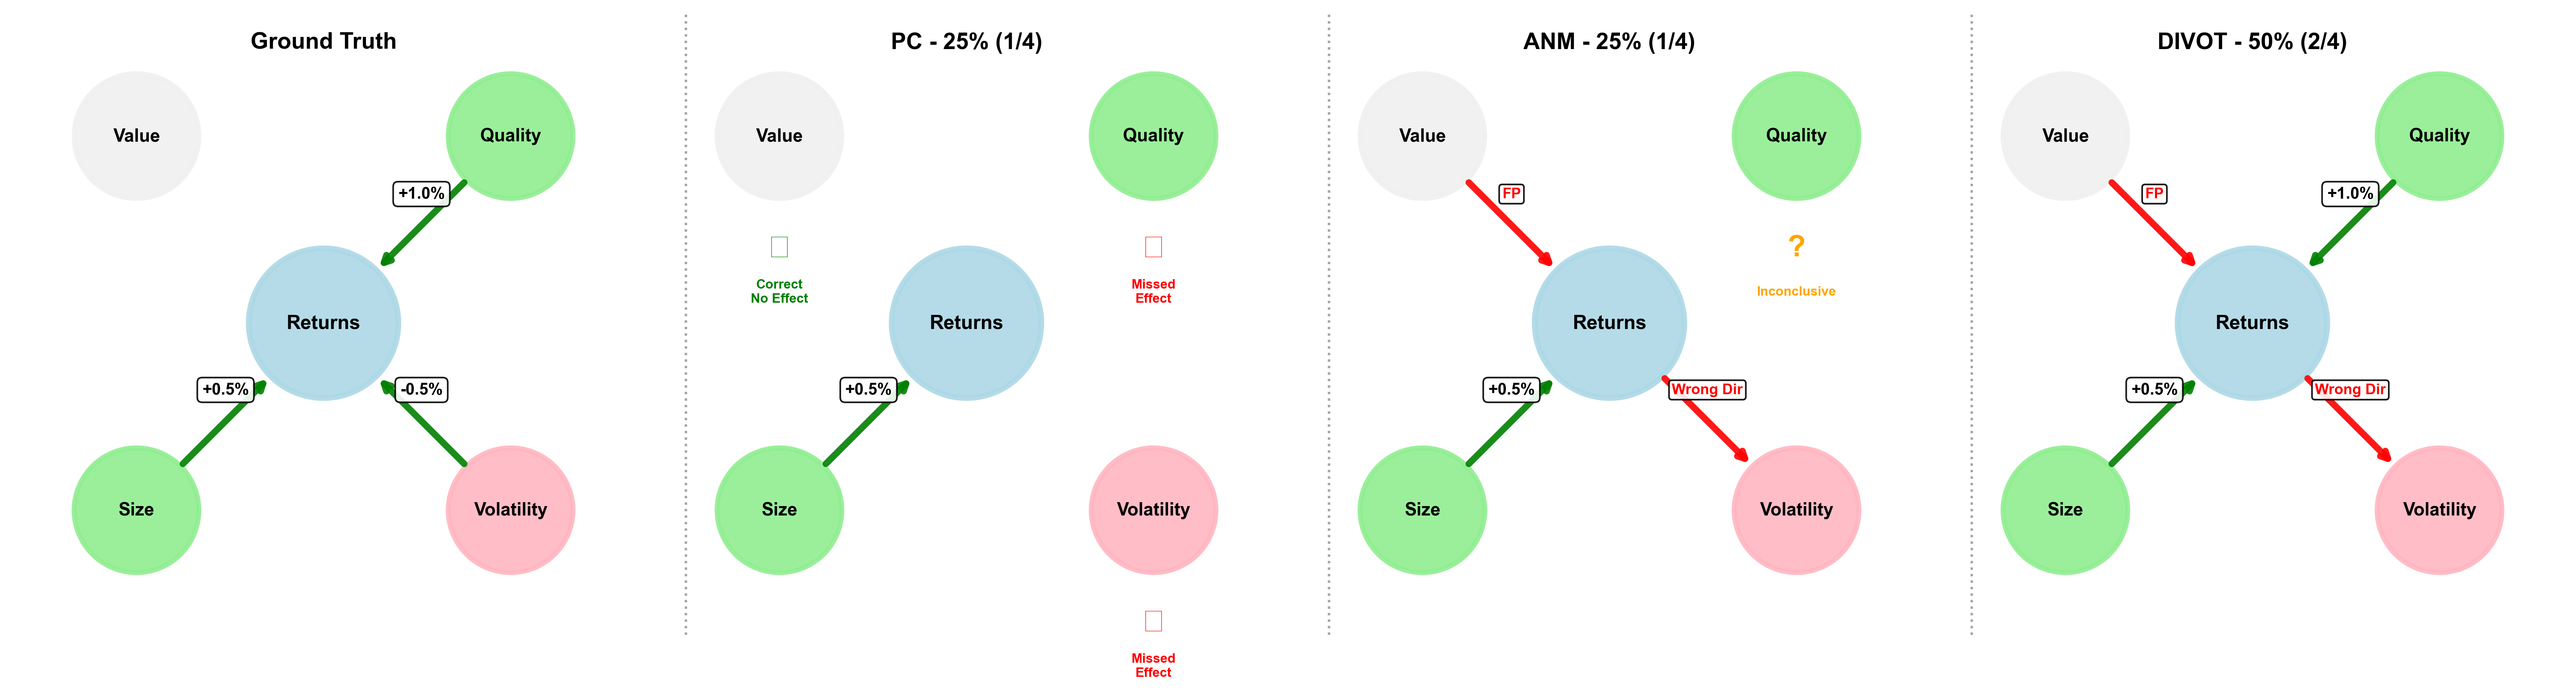
\includegraphics[width=\textwidth]{Graphs/Synthetic/detailed_causal_networks.png}
\caption{Comprehensive Causal Network Analysis, comparing the Ground Truth with the predictions from the DIVOT, ANM, and PC algorithms. The color-coding indicates correct (green) or incorrect (red) predictions for each factor relationship.}
\label{fig:all_method_comparison}
\end{figure}

% -------------------------------------------------------------------
\chapter{Appendix C: Real Data Analysis Summary}
\label{cha: Appendix C}

This appendix provides summary statistics and key results from our application of causal discovery methods to the Fama-French real financial data.

\section*{Data Processing Pipeline}
The final panel dataset was constructed from the raw Fama-French data files through a systematic process.
\begin{enumerate}
    \item \textbf{Loading Data}: We loaded the monthly returns for the 25 size/value sorted portfolios and the Fama-French-5 factors plus Momentum.
    \item \textbf{Date Filtering}: The data was filtered to include only the period from January 1990 to December 2023. This range was chosen to ensure data quality and consistency across all factors.
    \item \textbf{Duplicate Removal}: We scanned the data for duplicate entries, defined as a single portfolio having multiple return entries for the same month. These duplicates were removed to ensure each observation is unique.
    \item \textbf{Handling Missing Data}: Any rows with missing values for either portfolio returns or factor returns were removed from the dataset.
    \item \textbf{Panel Construction}: The cleaned data was then transformed from a time-series format into a panel structure, with each of the 25 portfolios treated as an individual unit observed over time.
\end{enumerate}
The final dataset contains \RealTotalObservations{} unique observations. This number is not equal to 25 portfolios multiplied by the number of months because some portfolios had missing data for certain periods in the raw data files.

\subsection*{Reproducibility Note}
The exact observation count in a replication of this study may vary slightly. This can be due to small differences in duplicate handling logic, the inclusion or exclusion of boundary dates, or the treatment of missing data. Our analysis uses a strict duplicate removal process and includes the full date range specified.

\section*{Data Overview}
\begin{table}[H]
    \centering
    \caption{Fama-French data characteristics. Data preprocessing included removal of duplicate portfolio-month observations and filtering to the 1990-2023 period to ensure data quality and consistency. The final panel contains \RealTotalObservations{} unique observations.}
    \begin{tabular}{|l|c|}
        \hline
        \textbf{Parameter} & \textbf{Value} \\
        \hline
        Data period & 1990 -- 2023 \\
        Number of months & 408 \\
        Number of portfolios & 25 (5$\times$5 size/value sorted) \\
        Panel observations & \RealTotalObservations{} \\
        Factors included & Mkt-RF, SMB, HML, RMW, CMA, WML \\
        Data source & Kenneth French Data Library\cite{FrenchData2024} \\
        \hline
    \end{tabular}
\end{table}

\section*{Factor Summary Statistics}
\begin{table}[H]
    \centering
    \caption{Monthly factor return statistics (1990-2023)}
    \begin{tabular}{|l|c|c|c|c|}
        \hline
        \textbf{Factor} & \textbf{Mean (\%)} & \textbf{Std Dev (\%)} & \textbf{Min (\%)} & \textbf{Max (\%)} \\
        \hline
        Market (Mkt-RF) & 0.71 & 4.44 & -17.20 & 13.58 \\
        Size (SMB)      & 0.12 & 3.04 & -15.54 & 18.46 \\
        Value (HML)     & 0.15 & 3.24 & -13.83 & 12.86 \\
        Momentum (WML)  & 0.42 & 4.71 & -34.30 & 18.00 \\
        Profitability (RMW) & 0.38 & 2.63 & -18.95 & 13.05 \\
        Investment (CMA)    & 0.20 & 2.18 & -7.08  & 9.01 \\
        \hline
    \end{tabular}
\end{table}

\section*{Causal Discovery Accuracy}
\begin{table}[H]
    \centering
    \caption{Causal discovery method performance on real data}
    \begin{tabular}{|l|c|c|}
        \hline
        \textbf{Method} & \textbf{Accuracy} & \textbf{Correctly Identified} \\
        \hline
        PC Algorithm & 1/6 (16.7\%) & RMW \\
        ANM   & 0/6 (0.0\%) & None \\
        DIVOT & 4/6 (66.7\%) & Market, SMB, HML, CMA \\
        \hline
    \end{tabular}
\end{table}

\noindent
The mixed results from the causal discovery methods on real data contrast sharply with their performance on synthetic data. This highlights the complexity of real financial markets where simple causal models are often insufficient. However, the methods still provide valuable insights. For example, the RMW factor was identified as causally relevant by multiple algorithms, even if they disagreed on the direction. This suggests it is a significant factor worthy of further investigation. None of the methods were able to correctly identify that returns drive the momentum factor, which highlights the challenge of detecting known feedback loops in noisy financial data.


% -------------------------------------------------------------------
\chapter{Appendix D: Code and Implementation}
\label{cha: Appendix D}

\section*{Code Availability}
All code, data processing scripts, and visualisation tools used in this thesis are publicly available at:

\begin{center}
\url{https://github.com/SaeedAnalysis/CausalityAndOTInFactorInvesting}
\end{center}

\section*{Repository Structure}
The repository is organised as follows:
\begin{itemize}
    \item \texttt{Python/Analysis/}: Core analysis scripts for synthetic and real data, including causal discovery implementations.
    \item \texttt{Python/Jupyter/}: Jupyter Notebook versions of the core analysis scripts for interactive exploration.
    \item \texttt{Python/Graphs/Generation Scripts/}: Scripts for generating all figures and plots.
    \item \texttt{Real\_Data/}: Fama-French data files and associated data-loading functions.
    \item \texttt{Graphs/}: Output directory containing all generated figures.
    \item \texttt{Overleaf/}: LaTeX source files for the thesis.
    \item \texttt{requirements.txt}: Python package dependencies.
\end{itemize}

\section*{Reproducibility}
To reproduce the analysis:
\begin{enumerate}
    \item Clone the repository
    \item Ensure Python 3.8+ is installed
    \item Install dependencies: \texttt{pip install -r requirements.txt}
    \item Run the main analysis scripts:
    \begin{itemize}
        \item \texttt{python Python/Analysis/Causality\_Main.py} (synthetic data)
        \item \texttt{python Python/Analysis/Causality\_Real\_Data.py} (real data)
    \end{itemize}
\end{enumerate}

\section*{System Requirements}
\begin{itemize}
    \item \textbf{Python Version}: 3.8 or higher (tested with Python 3.9 and 3.10)
    \item \textbf{Key Dependencies}: numpy, pandas, scikit-learn, causal-learn, POT (Python Optimal Transport)
    \item \textbf{Memory}: Minimum 4GB RAM (8GB recommended for large datasets)
    \item \textbf{Storage}: 500MB for code and data files
\end{itemize}

The repository includes both synthetic data generation and real data analysis pipelines, allowing full replication of all results presented in this thesis.

\printindex
\end{document}